\documentclass{indc-report}
\setlength{\headheight}{15pt}

% Publication number, DOI and preparers have not been confirmed.
\newcommand{\reportnumber}{INDC-NDS-xxxx}
\newcommand{\reportdistribution}{Draft}
\newcommand{\reportdoi}{}
\newcommand{\reportdate}{30 October 2026}
\newcommand{\reportpreparer}{
                            Dragan Avramovski, Arjan Koning, Alejandra Martinez, Shin Okumura, Georg Schnabel\\
                            IAEA Nuclear Data Section\\
                            ~\\
                            Anastasia Georgiadou, Julia Sprenger\\
                            OECD/NEA Data Bank\\
                            ~\\
                            Yukari Katsura\\
                            National Institute for Materials Science, Japan\\
                            ~\\
                            Donnie Mason\\
                            Brookhaven National Laboratory, USA\\
                            }

\newcommand{\meetingdate}{27--30 October 2026}
\newcommand{\meetinglocation}{IAEA Headquarters, Vienna, Austria}
\newcommand{\meetingplace}{Room M0E13}
\newcommand{\meetingtype}{Consultancy Meeting}
\newcommand{\meetingsubject}{Follow-up Developments in Nuclear Data Retrieval, Dissemination, and Data Portal}
\title{Summary Report of the \meetingtype\ on \meetingsubject}

\begin{document}
%%% First page - cover title

{
\pagestyle{empty}
% Full-width cover boxes must not reserve a 30pt paragraph-end space.
\setlength{\parfillskip}{0pt plus 1fil}
% \thispagestyle{empty}
\thispagestyle{firstpage}
%%\newgeometry{top=2cm, bottom=2.5cm, left=2.5cm, right=2.5cm}

\noindent\begin{minipage}{.6\textwidth}
  
\includegraphics[width=220pt]{figures/standart-Logo-E_horizontal_K.pdf}
\end{minipage}%
\begin{minipage}{.4\textwidth}
  {\normalfont\sffamily\bfseries\flushright\fontsize{12pt}{0pt}\selectfont
  \reportnumber \\
  Distr. \reportdistribution \\}
\end{minipage}

{\normalfont\sffamily\bfseries\fontsize{20pt}{10pt}\selectfont
  INDC International Nuclear Data Committee\\
}

\begin{center}
  {\normalfont\sffamily\fontsize{16pt}{60pt}\selectfont
    Summary Report of the \meetingtype\ on the\\
  }

  {\normalfont\sffamily\bfseries\fontsize{18pt}{36pt}\selectfont
      \meetingsubject \\
  }
  {\normalfont\sffamily\fontsize{14pt}{24pt}\selectfont
    \meetinglocation \\
    \meetingdate \\
  }
%  \bigskip
%  \bigskip
%  \bigskip
%  \bigskip
   \vskip1.5\baselineskip
    {\normalfont\sffamily\fontsize{20pt}{10pt}
      \bigskip
      \reportpreparer\par
      \bigskip
      \reportdate \\
    }
%   \vspace{6cm}
    \vfill
     {\normalfont\sffamily\fontsize{12pt}{20pt}\selectfont
       \hrulefill \\
       IAEA Nuclear Data Section\\
       Vienna International Centre, P.O. Box 100, 1400 Vienna, Austria\\
       \hrulefill
     }
\end{center}
\newpage

%%% Second page - INDC document reference

\thispagestyle{empty}
\noindent\begin{minipage}{1.0\textwidth}
  \vspace{15cm}
  \begin{center}
    Selected INDC documents may be downloaded in electronic form from\\
    \url{http://nds.iaea.org/publications}\\
    or sent as an e-mail attachment.\\
    Requests for hard copy or e-mail transmittal should be directed to\\
    NDS.Contact-Point@iaea.org\\
    or to:\\
    Nuclear Data Section\\
    International Atomic Energy Agency\\
    Vienna International Centre\\
    PO Box 100\\
    1400 Vienna\\
    Austria\\
    \bigskip
    \bigskip
    Printed by the IAEA in Austria\\
    \bigskip
    \reportdate \\
  \end{center}
\end{minipage}
\newpage

%%% Third page - inside cover and abstract

\thispagestyle{empty}
\noindent\begin{minipage}{.6\textwidth}
 ~ \\
\end{minipage}%
\begin{minipage}{.4\textwidth}
  {\normalfont\sffamily\bfseries\flushright\fontsize{12pt}{0pt}\selectfont
  \reportnumber \\
  Distr. \reportdistribution\\}
\end{minipage}

\begin{center}
  {\normalfont\sffamily\fontsize{14pt}{40pt}\selectfont
    Summary Report of the \meetingtype\ on the\\
  }

  {\normalfont\sffamily\bfseries\fontsize{16pt}{36pt}\selectfont
    \meetingsubject \\
  }

  {\normalfont\sffamily\fontsize{12pt}{24pt}\selectfont
    \meetinglocation \\
    \meetingdate \\
  }
\bigskip
  {\normalfont\sffamily\fontsize{20pt}{10pt}
    \bigskip
    \medskip
    \reportpreparer
  }
\end{center}
%\vspace{6cm}
\vfill
\bigskip
\begin{abstract}
This report records the Consultancy Meeting on Follow-up Developments in Nuclear Data Retrieval, Dissemination, and Data Portal, held at IAEA Headquarters on 27--30 October 2026. It covers nucelar data retrieval services, processing tools, experimental data submission, ENSDF modernisation and curation of published data. The discussions concern shared software, reproducible processing, metadata and practical connections between developers and users. 

The meeting presentations are available at: \url{https://conferences.iaea.org/event/498/}.




\end{abstract}
\bigskip
\begin{center}
\reportdate
\end{center}
\newpage

%%% Table of contents

\thispagestyle{empty}
\mbox{}\newpage

\thispagestyle{empty}
\begin{spacing}{1.5}
\setlength{\emergencystretch}{2em}
\addtocontents{toc}{\protect\thispagestyle{empty}}
\tableofcontents
\thispagestyle{empty}
\end{spacing}
\newpage
}

\restoregeometry


\section{Introduction}
The Consultancy Meeting on ``Follow-up Developments in Nuclear Data Retrieval, Dissemination, and Data Portal'' is being held at IAEA Headquarters, Vienna, on 27--30 October 2026, in Room M0E13. It follows the Technical Meeting of November 2024 and reviews developments in retrieval, dissemination and portal services~\cite{meeting498,report2024}. The meeting opened with welcome addresses by A.~Koning, Head of the Nuclear Data Section, and S.~Okumura, Scientific Secretary.

The meeting provides a small, interactive forum for developers and users to exchange implementation experience, demonstrate tools and identify opportunities for collaboration. Its programme covers IAEA Nuclear Data Section, OECD/NEA Data Bank, and Brookhaven National laboratory (BNL) developments, processing and conversion tools, data-submission workflows and applications of machine learning and local language models (LLM).

Presentations and discussions covered four related areas:
\begin{itemize}
    \item Nuclear data retrieval, visualization and dissemination services, including web interfaces and APIs;
    \item Processing, conversion, validation and evaluation workflows for experimental and evaluated nuclear data;
    \item Data schemas, metadata, submission workflows, provenance, versioning and persistent identifiers;
    \item AI/ML-assisted data curation, quality assessment and agentic workflows.
\end{itemize}
Participants exchanged implementation experience and discussed interoperability, reuse of software and continued collaboration between developers. Examples of user requests and the responses of service developers provided a practical basis for these discussions.
 

The presentation materials are available at:
\begin{center}
    \url{https://conferences.iaea.org/event/498/}
\end{center}


\newpage

\section{Presentation summaries}

\subsection{Tuesday, 27 October 2026}

\subsubsection{Nuclear Data Retrieval, Dissemination, and Data Portals\\ Shin Okumura (IAEA)}
% Official contribution: https://conferences.iaea.org/event/498/contributions/43608/
% Scheduled date: 2026-10-27.
\paragraph{Abstract}
\textit{The Consultancy Meeting on Follow-up Developments in Nuclear Data Retrieval, Dissemination, and Data Portal\ldots}

This introductory presentation outlines the role of nuclear data dissemination in connecting experimental measurements, evaluated libraries and applications. It distinguishes the needs of evaluators, experimental and theoretical physicists, nuclear engineers and application users, and introduces the complementary resources of the IAEA Nuclear Data Section, OECD/NEA Data Bank and Brookhaven National Laboratory's National Nuclear Data Center.

Effective dissemination requires expertise in data management, software engineering and modern data technologies alongside nuclear physics. Building on the meetings held in January and November 2024~\cite{report2024}, this consultancy meeting reviews progress, shares ongoing developments and explores opportunities for collaboration among developers and data management specialists. Topics include retrieval and visualisation, APIs, data processing, interoperability and emerging technologies. The emphasis is on connecting the people who make nuclear data accessible and usable, exchanging practical experience and learning from other scientific communities. An open, constructive working environment is intended to support knowledge sharing and strengthen continued collaboration across institutions.



\paragraph{Discussion}
% Source: Webex-Summary/day2.pdf; use the meeting date, not the filename.
Shin Okumura outlined the meeting's practical focus and the relationship between compilation, evaluation, dissemination and applications. Discussion addressed differing user needs and the complementary services of the participating centres. Participants considered how shared components, interfaces and development experience and practices could make better use of limited human workloads. The meeting was framed as an opportunity to connect ongoing work and test possible improvements through demonstrations and open discussion.


\subsubsection{Updates on IAEA Nuclear Reaction DataExplorer Developments\\ Shin Okumura (IAEA)}\label{Pres:SO2} 
% Official contribution: https://conferences.iaea.org/event/498/contributions/43620/
% Scheduled date: 2026-10-27.
\paragraph{Abstract}
This presentation reviews the modernisation of IAEA Nuclear Data Dissemination Services, focusing on the Nuclear Reaction Data Explorer \url{https://nds.iaea.org/dataexplorer} and its supporting workflows~\cite{dataexplorer}. The backend converts EXFOR records into JSON~\url{https://github.com/IAEA-NDS/exfor_json} and SQL database, and tabulated data files~\cite{EXFORTABLES-py} for retrieval and visualisation (Figure~\ref{fig:so-dataflow}). Developments include broader observable coverage, visualization of various observables, library comparisons, access to historical evaluations powered by DeCE code~\cite{Kawano2019DeCE} (Figure~\ref{fig:so-dece}), bibliographic and reaction-index searches for EXFOR entries, (Figure~\ref{fig:so-stat}) and APIs.
\begin{figure}[htbp]
    \centering  
    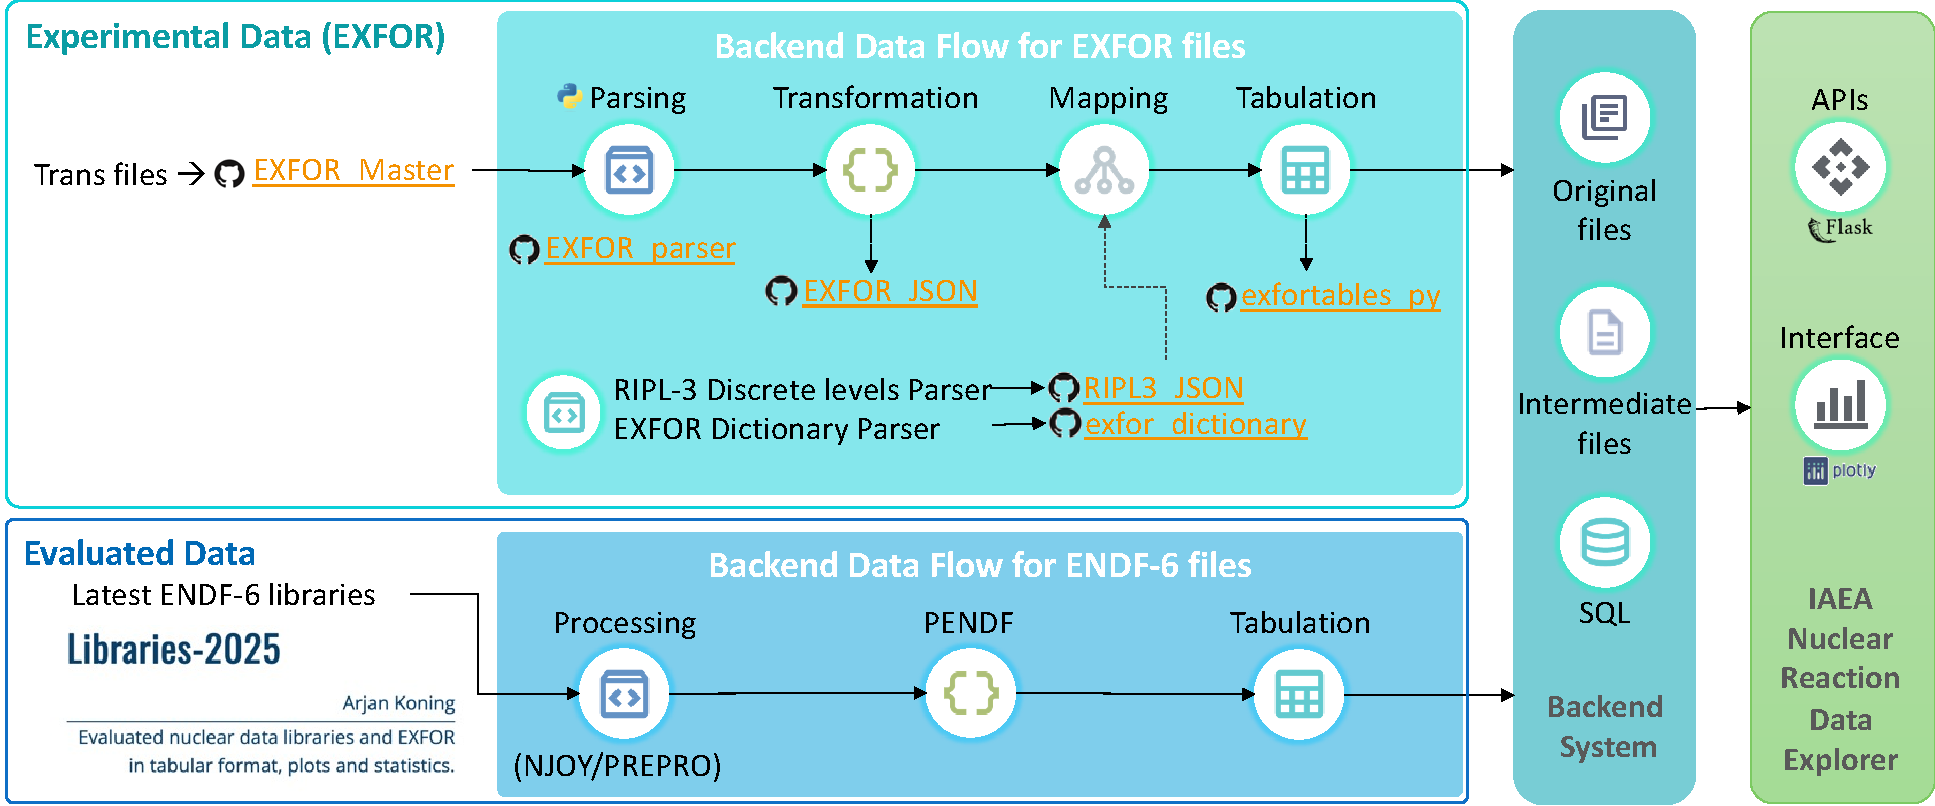
\includegraphics[width=0.6\textwidth]{figures/okumura-dataflow.pdf}
    \caption{Dataflow: Experimental (EXFOR) and Evaluated (ENDF-6) Data}
    \label{fig:so-dataflow}
\end{figure}
\begin{figure}[htbp]
    \centering  
    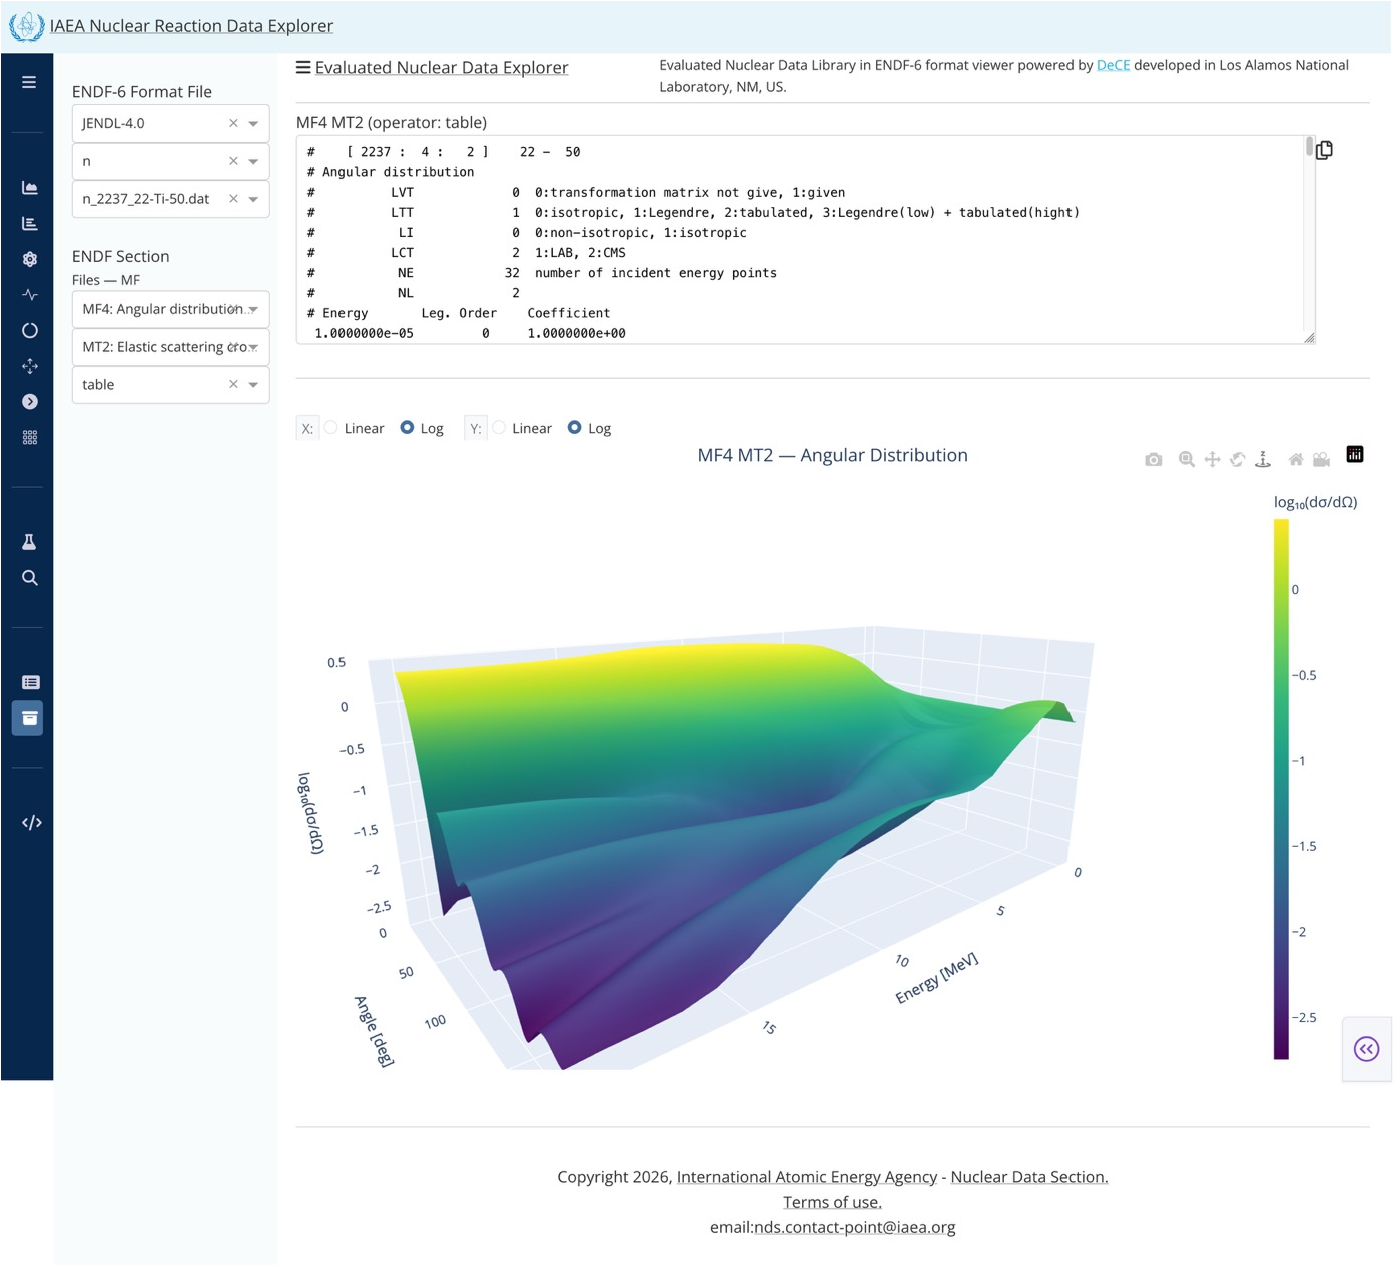
\includegraphics[width=0.6\textwidth]{figures/okumura-dece.pdf}
    \caption{Access to historical evaluations powered by DeCE code~\cite{Kawano2019DeCE}}
    \label{fig:so-dece}
\end{figure}
\begin{figure}[htbp]
    \centering  
    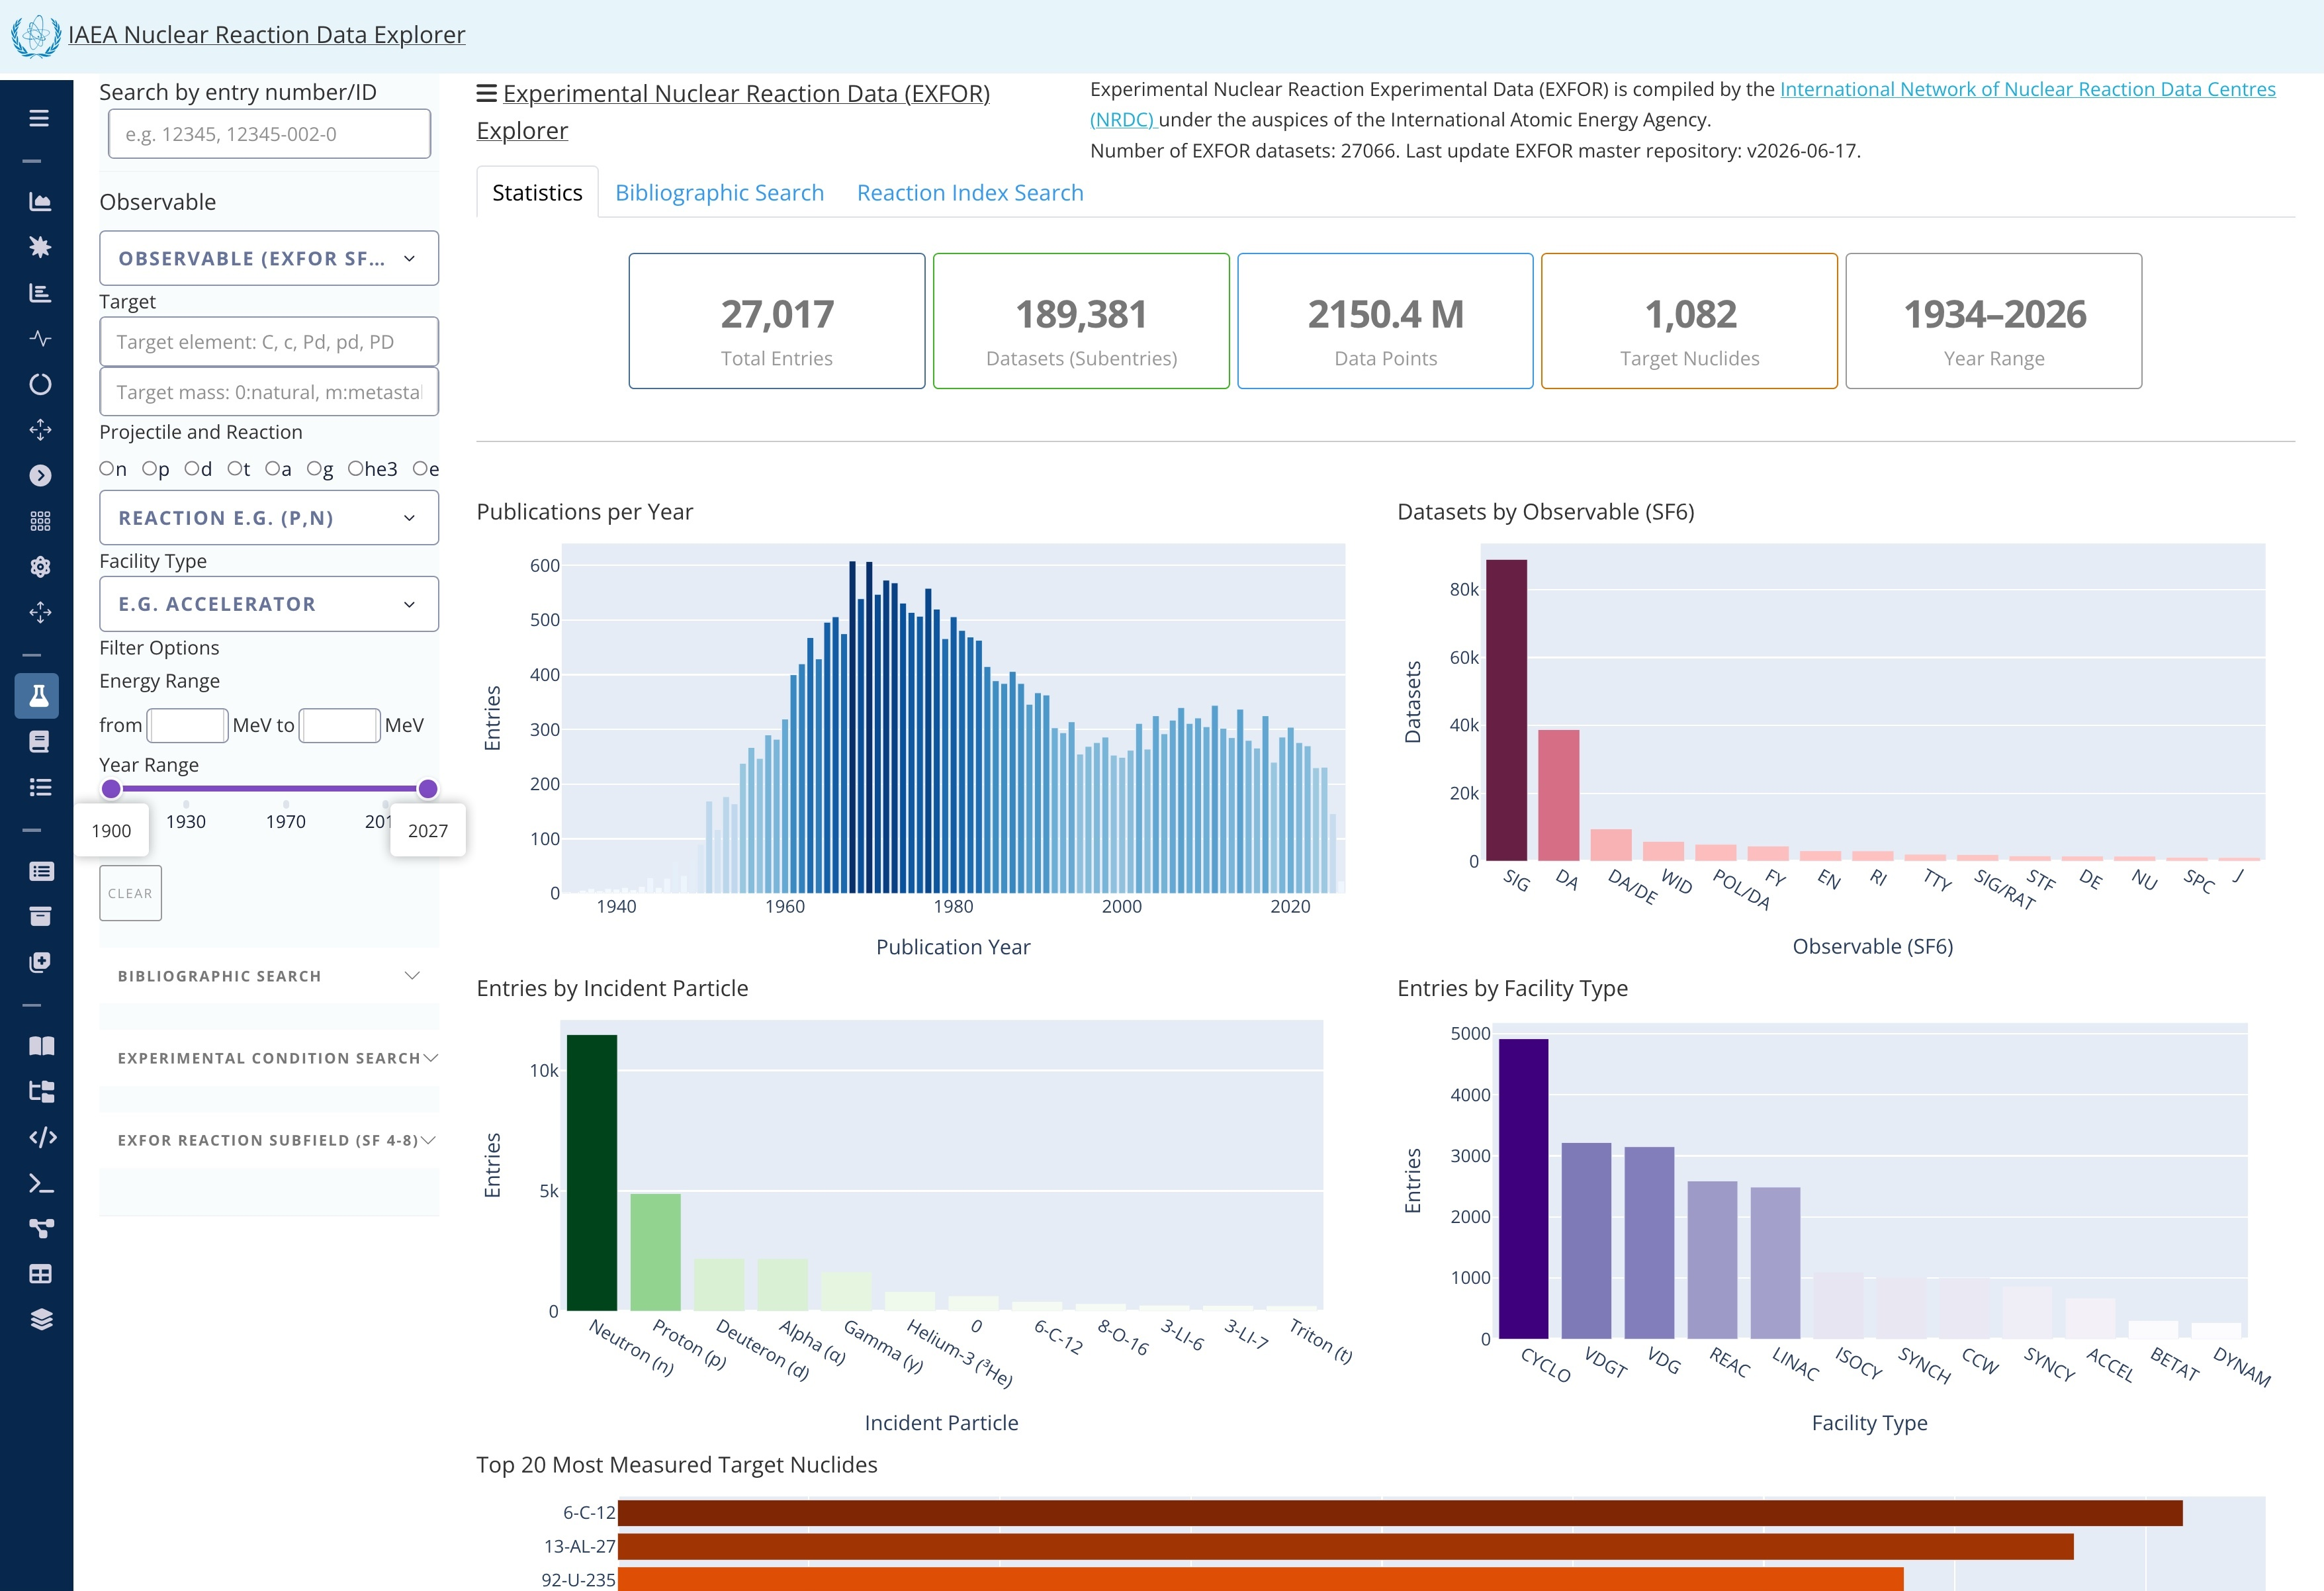
\includegraphics[width=0.75\textwidth]{figures/okumura-exfor-statistics.jpg}
    \caption{EXFOR Statistics}
    \label{fig:so-stat}
\end{figure}


A complementary workflow recovers missing publication DOIs from EXFOR bibliographic information~\cite{exfor-entry-doi}. It uses title and author matching through Crossref, together with lookup rules for coded journal and report references. The scope includes main references, related references and monitor references. Existing identifiers are preserved, and the source of entry-level additions is recorded. Similarity-based matches remain heuristic and require stronger bibliographic checks and review of ambiguous candidates.

The presentation also introduces a community-contribution prototype on Data Portal Project linking submitted or revised datasets to publications and EXFOR records, and tests of migrating legacy NDS resources to Invenio~\cite{invenio}. These developments address data discovery, provenance, reuse and long-term maintenance. Further work includes production deployment, automated updates, completeness checks, moderation workflows and verification that migration preserves data and associated resources.
\mbox{}\par

\paragraph{Discussion}
Shin Okumura demonstrated Data Explorer's access to experimental and evaluated data through parsed records, tabulated observables, plots and APIs. Discussion covered filtering, library comparisons, plot controls and links back to source records. 

Participants also suggested comparison with users' local data, including browser-side handling and temporary uploads. Storage, authentication and review arrangements for a broader submission service remained open until the IAEA officially provides new SSO service such as NUCLEUS. 

\subsubsection{Strengthening Collaboration and Reproducibility in the Nuclear Data Community: Challenges and NEA Initiatives\\ Julia Sprenger (OECD/NEA)}
% Official contribution: https://conferences.iaea.org/event/498/contributions/43621/
% Scheduled date: 2026-10-27.
% Official description is "TBD"; treated as no abstract.
\paragraph{Abstract}
% No substantive abstract published at the time of preparation.
This presentation provides an overview of recent developments at the NEA Data Bank for 3 different topics around international collaborations and project management.

First topic are the conceptual requirements for a collaboration in the 21st century. Key requirements identified are transparency, and tracability of contributions, persistence of releases as well as common project management practices and data structures. Examples are provided from the recent NEA SCI project modernisation.

Secondly, the need for open data standards and facilitated data contribution to international projects has been identified as key requirements. Recent implementations on this from the NEA are an Exfor Submission Form (more details in \ref{subsec:EXFOR_Streamlined}).  

As third topic, persistent identifiers and integration into field-specific resource networks are identified as essential to make resources findable and accessible via standard interfaces. Here, the NEA DB launched an InvenioRDM instance which integrates records into the DataCite framework, providing DOIs and interlinking with related resources.

Finally, the presentation triggered discussions on community practices, sustainability, project ownership and future developments paths of legacy tools and datasets and new developments.

\mbox{}\par

\paragraph{Discussion}
% Source: Webex-Summary/day2.pdf; use the meeting date, not the filename.
% Also checked against published slides; do not attribute later JADE/git-annex discussion here.
Julia Sprenger's contribution described NEA initiatives for tracking contributions, community ownership and persistent releases~\cite{neaSlides}. Modular schemas and automated conversion, validation and documentation were presented as building blocks shared between projects. Discussion concerned making collaboration through Git easier for users unfamiliar with these tools and connecting repositories, APIs and user-facing services. The EXFOR form illustrated a contribution pathway still requiring decisions on authentication and backend integration. The public slides also acknowledge Anastasia Georgiadou.


\subsubsection{EXFOR Streamlined Reaction Data Submission\\ Anastasia Georgiadou and Julia Sprenger (OECD/NEA)}\label{subsec:EXFOR_Streamlined}
% Official contribution: https://conferences.iaea.org/event/498/contributions/43613/
% Scheduled date: 2026-10-27.
\paragraph{Abstract}
\textit{Building an EXFOR~\cite{EXFOR} submission template and early community feedback}

This talk presents the development of a structured submission template to streamline experimental nuclear reaction data submission to EXFOR \url{https://exfor.io.oecd-nea.org/template/}. The approach addresses ambiguous metadata, inconsistent uncertainty descriptions, and missing experimental context that complicate compilation and reuse. Structured fields and defined uncertainty categories aim to preserve the scientific meaning of measurements while reducing manual interpretation. The template integrates into a collaborative GitLab workflow \url{https://git.oecd-nea.org/exfor} that supports traceable data submission, metadata review and validation before EXFOR compilation. A JSON Schema prototype, built on the NSC WPEC SG50~\cite{SG50-2023} framework, provides the basis for specifying the required information. Examples illustrate how the proposed format capture’s reaction details, bibliographic information, measured values, and associated uncertainties. A functional submission form and workflow prototype demonstrate progress towards direct contributions from experimentalists and automated processing. The presentation also discusses early community feedback gathered at WINS 2026 in Geel, Belgium~\cite{WINS2026}. This consultation explores information requirements, submission priorities, and preferences for the template’s structure. Further development will focus on modularisation, validation, and community testing, alongside agreement on mandatory fields and unresolved expert questions. The overall aim is to reduce compilation effort while keeping experimental knowledge complete, interpretable, and reusable.

\begin{figure}[htbp]
    \centering  
    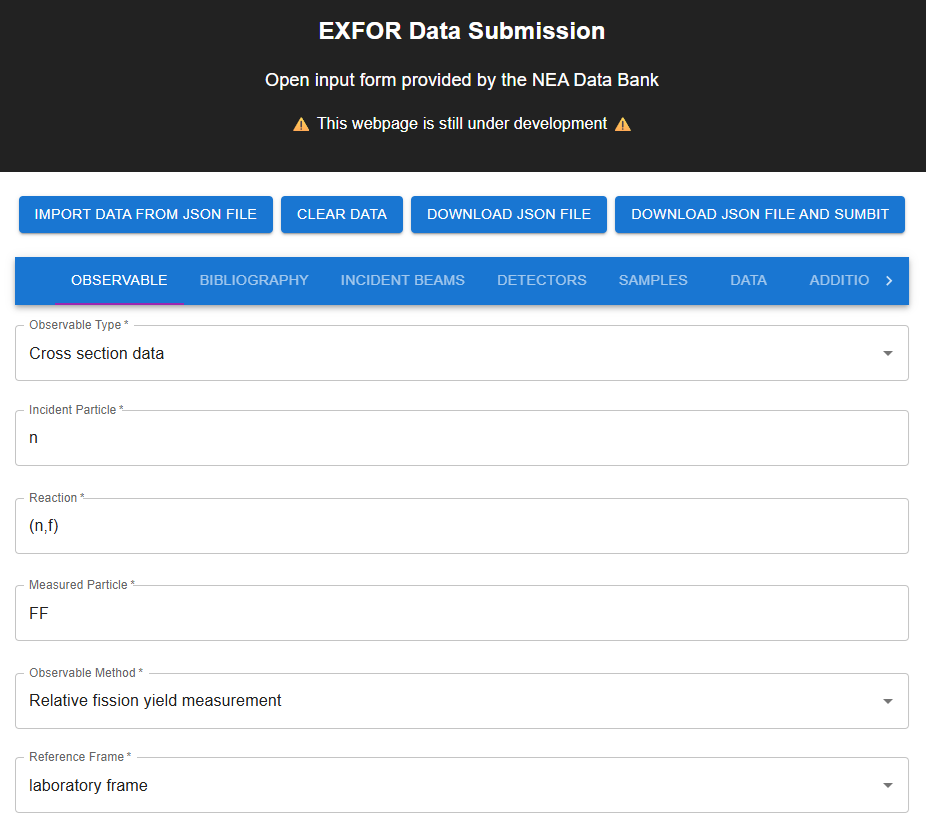
\includegraphics[width=0.8\textwidth]{figures/exfor_template_submission.png}
    \caption{Screenshot of the preliminary EXFOR Submission Form.}
    \label{fig:submission_form}
\end{figure}


\paragraph{Discussion}
% Source: Webex-Summary/day2.pdf; use the meeting date, not the filename.
Anastasia Georgiadou described a submission form backed by a schema and a GitLab workflow. Discussion covered mandatory metadata, copying tabulated values from existing tools, modular forms and reducing repeated entry. Participants raised the need to describe systematic uncertainties and correlations beyond simple per-point columns, together with reference standards and experimental context. Community feedback would inform further testing. A direct automated ingestion service was discussed as future work; the demonstrated workflow retained validation and human review before compilation.


\subsubsection{Autotalys nuclear data pipeline with GitHub, ChatGPT and Codex\\ Arjan Koning (IAEA)}
% Official contribution: https://conferences.iaea.org/event/498/contributions/43618/
\paragraph{Abstract}
The AutoTALYS~\cite{autotalys} pipeline presented here aims to bring experimental nuclear reaction 
measurements from EXFOR~\cite{EXFOR} and theoretical calculations from TALYS~\cite{Koning2023TALYS} into a common workflow. 
It supports the production of TENDL~\cite{TENDL} and related evaluated libraries, optimization of nuclear model parameters, 
astrophysical cross sections and reaction rates, medical isotope data, and the calculation of uncertainties, 
covariance matrices, and sensitivity profiles. 
This presentation describes how a Git based collection of codes and databases can make those activities easier to 
install, reproduce, inspect, and extend. It also examines the role of ChatGPT and Codex in developing software for 
the pipeline, while keeping scientific choices and review with the nuclear data specialist.

AutoTALYS is assembled from repositories with distinct functions. 
TALYS calculates nuclear reactions; TEFAL~\cite{tefal} converts results into ENDF-6~\cite{ENDF6FormatsManual2023} evaluations; 
TASMAN handles optimization, sensitivity, covariance, and Total Monte Carlo calculations. 
Supporting codes address isotope production, normalization, and ENDF-6 validation and processing. 
Other repositories hold experimental tables, resonance information, fission data, and specialized cross-section libraries. 
Installation scripts and a central workflow driver connect these components. 
The Git based structure provides a practical way to obtain the system and trace changes in its codes and inputs. 
For a data portal, this structure matters because a displayed value is more useful when its underlying measurement, 
calculation, transformation, and evaluation can be found and examined.

The EXFOR workflow illustrates that connection. An EXFOR JSON parser~\cite{EXFORParser} supplies entries, reactions, measurements, 
and metadata. Conversion software normalizes the measurements into tables and organizes them by projectile, nuclide, 
category, reaction, and dataset. Evaluator annotations from a separate outlier repository are matched to the 
experimental records. This produces a directory structured database that retains measured points alongside 
their metadata and subjective quality assessments. The outlier repository contains more than 20,000 files, 
representing a substantial body of manual review. Preserving these annotations with the numerical data allows 
later analyses to use expert judgment without obscuring where that judgment came from.

Automated analysis adds another layer of evidence. A Codex generated quality score considers data integrity, 
reported uncertainties, consistency with peer experiments, provenance, and metadata; 
eligible total cross sections may also be compared with evaluated libraries. 
The score starts at 0.50, applies specified rewards and penalties, and is bounded between zero and one. 
A higher value indicates stronger evidence under these rules, rather than proof that a dataset is correct. 
The presentation notes a current limitation: uncertainties below 0.1\% are not flagged as implausibly small 
by the scoring rule. A separate outlier comparison examines peer experiments and library curves against 
manual outlier judgments. It does not take the Codex quality score as an input. Keeping the automated score, 
comparison result, and evaluator annotation distinct makes disagreements visible and gives reviewers a clearer 
basis for investigation.

The same approach extends to low energy neutron data through the resonancetables repository~\cite{resonancetables}. Its purpose is to 
gather existing compilations and evaluations of thermal cross sections, Maxwellian averaged cross sections, 
resonance integrals, average resonance parameters, and individual resonance parameters. 
The material draws on EXFOR, established atlases and compilations, and major evaluated libraries, 
including ENDF/B-VIII.1~\cite{ENDFB8.1}, JEFF-4.0~\cite{JEFF40}, JENDL-5.0~\cite{Iwamoto2023JENDL5}, and TENDL-2025~\cite{TENDL}. 
The immediate task is a compilation of those sources; an evaluation across the collected compilations remains 
a further step. Bringing them together should make both automated and manual evaluation more efficient by 
exposing differences among sources and reducing repeated data gathering. 
An example for the thermal capture cross section of osmium-190 shows how EXFOR parsing can support this comparison.

Quality assessment also has a broader, library-wide dimension. The presentation reports a horizontal comparison 
using an Frms measure for several evaluated libraries, with values close to unity: 
1.034 for CENDL-3.2, 1.020 for JENDL-5.0, 1.021 for ENDF/B-VIII.1, 1.011 for TENDL-2025, 1.024 for JEFF-3.3, and 
1.015 for JEFF-4.0. Such summary measures help identify overall agreement with selected experimental data, 
but their interpretation depends on dataset selection, quality decisions, and the reactions included. 
The workflow therefore retains dataset level statistics and provenance rather than relying on a single aggregate number. 
Examples of plotted cross sections and detailed dataset records demonstrate how numerical comparisons can lead 
back to individual measurements and their evaluation context.

Model adjustment provides the next connection between retrieval and production. 
TASMAN~\cite{tasman} already automates TALYS parameter optimization, and the pipeline has generated covariance data and linear 
sensitivity coefficients across nuclides. The proposed development is to optimize TALYS against all relevant reaction 
channels with curated EXFOR data at once, concentrating on approximately twenty of the most sensitive parameters. 
The presentation also proposes adding a non-model evaluation above the resonance range, with TENDL-2027 as the target. 
These are planned capabilities, distinct from the functions already demonstrated. Their success will depend on the 
quality and coverage of the experimental inputs, defensible treatment of uncertainty, and careful review of 
conflicts among reaction channels.

The central lesson for nuclear data dissemination is that a portal can serve as an entry point to a traceable evaluation 
process. Git based installation, structured experimental tables, retained human annotations, explicit automated scores, 
library comparisons, and model sensitivity information give users ways to understand how a result was reached. 
ChatGPT and Codex have helped clean up installation procedures and generate analysis and plotting code, with 
further agent driven workflows envisaged. The presentation reports gains in TALYS speed and memory economy, 
alongside improved portability. These developments can accelerate the handling of large and diverse nuclear data 
collections. Scientific oversight remains essential: specialists must frame the questions, check whether generated 
outputs make physical sense, and decide how evidence should influence an evaluation. The resulting direction is a 
connected nuclear data pipeline in which retrieval, quality assessment, model calculation, 
and dissemination reinforce one another.


\paragraph{Discussion}
% Source: Webex-Summary/day2.pdf; use the meeting date, not the filename.
Arjan Koning described an automated reaction-data pipeline combining experimental inputs, model calculations, optimisation and derived products. Versioned repositories and installation scripts were intended to make the workflow easier to reproduce. Discussion addressed dataset annotations, automated scoring and the treatment of outliers. Participants distinguished heuristic scores from documented reasons for accepting or excluding measurements, and considered fixed, testable routines as a way to make AI-assisted development reproducible. Large covariance products, model limitations and the distribution of generated data remained practical challenges.


\subsubsection{Progress in the Development of the New Nuclear Data Retrieval System\\ Alejandra Martinez (IAEA)}
% Official contribution: https://conferences.iaea.org/event/498/contributions/43617/
% Scheduled date: 2026-10-27.
\paragraph{Abstract}
The objective of this presentation is to provide an overview of the architecture and progress of the new dissemination system, with a focus on the pipelines developed in Python for EXFOR data extraction, alongside with the use of NJOY~\cite{NJOY}, endf-parserpy~\cite{endf-parserpy} and endf-userpy~\cite{endf-userpy} for processing evaluated nuclear data in ENDF-6 format~\cite{ENDF6FormatsManual2023}. These pipelines are designed to extract, process, and store nuclear observables from EXFOR and ENDF into a unified retrieval system, enabling their discovery, visualization and comparison through a common interface.

The system adopts a modular approach that decouples the data processing, storage, retrieval services, and presentation layer, seeking to improve maintainability, scalability, and extensibility.

The presentation will highlight the progress achieved, current challenges, and next steps towards a nuclear reaction data platform that is better aligned with the FAIR principles.


\paragraph{Discussion}
Alejandra Martinez demonstrated the new nuclear data retrieval system, combining experimental and evaluated data into nuclear observables, standardised units and a common interface. The demonstration included filters, library overlays, plot controls and downloads linked to original records. Discussion addressed observable definitions, precomputed and on-demand processing, and provenance in exported data. Participants identified reaction-string interpretation and display utilities as candidates for sharing between centres. Local-agent queries were exploratory; user-upload comparisons and some detailed views are items considered to be developed in the future.

\begin{figure}[H]
    \centering
    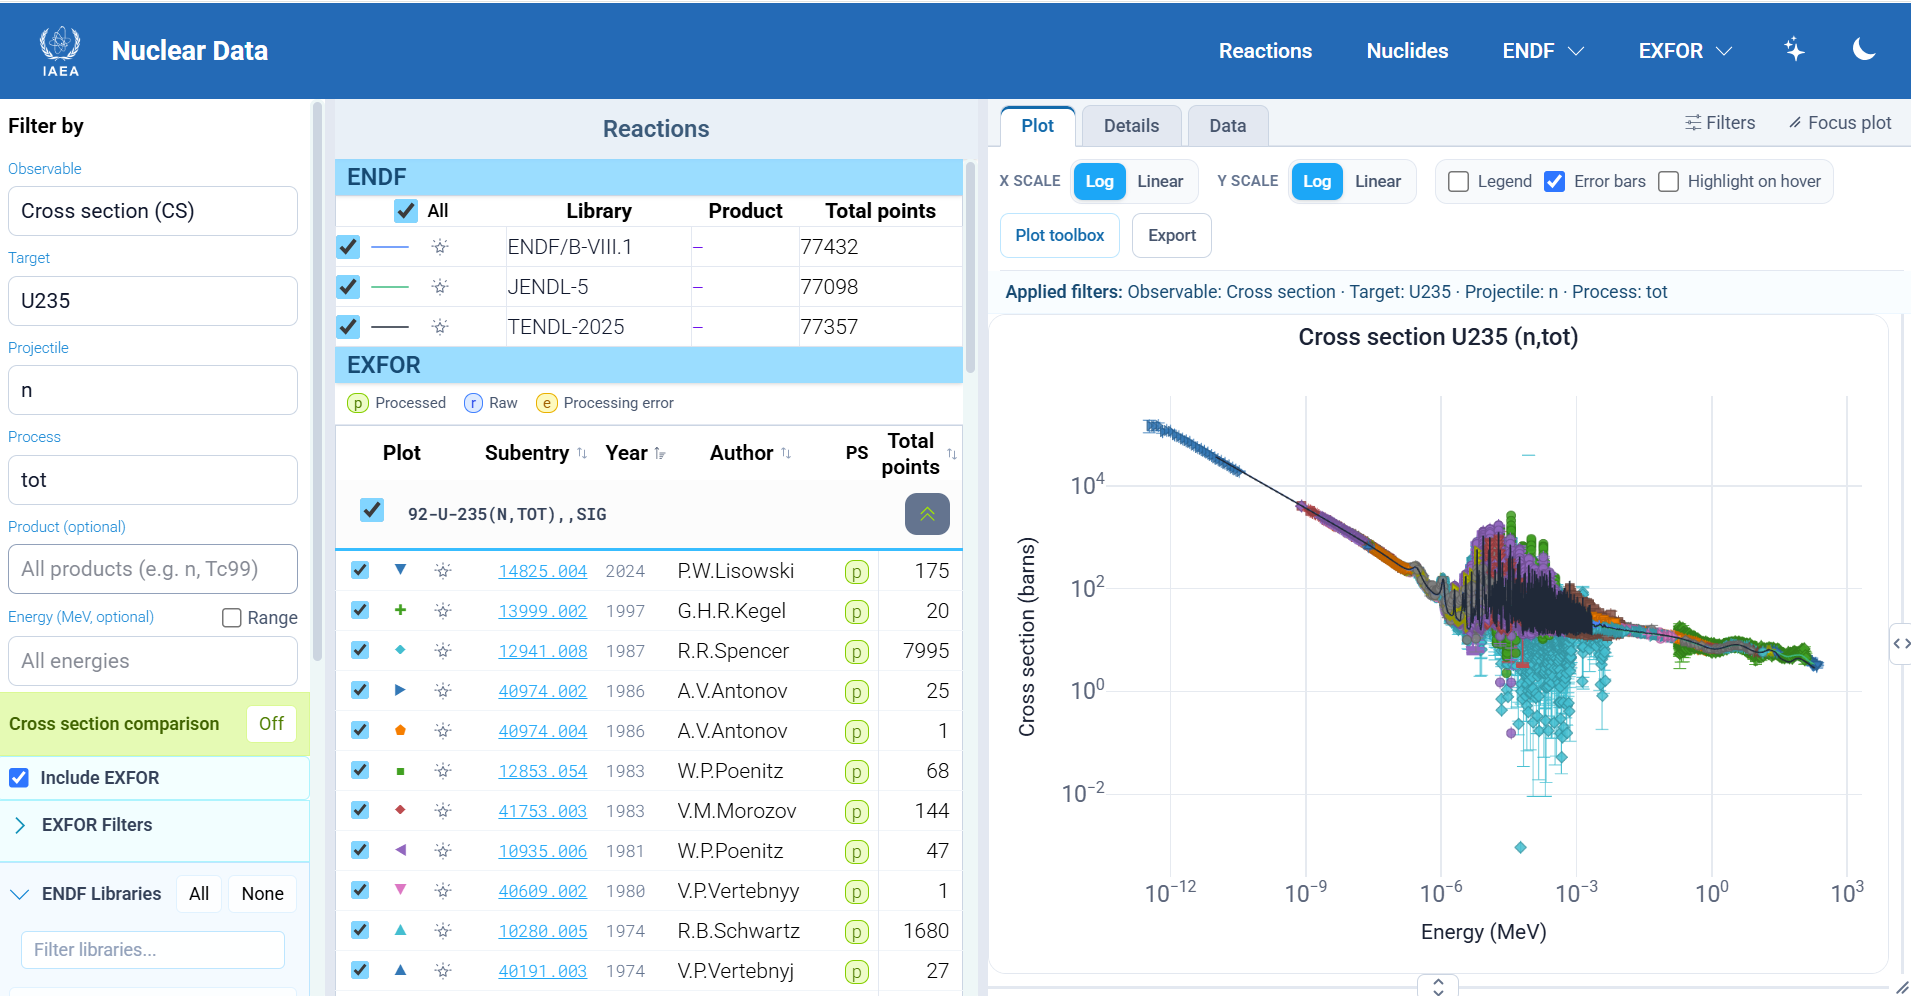
\includegraphics[width=0.75\linewidth]{figures/Screenshot 2026-10-29 144946.png}
    \caption{Screenshot of the New Nuclear Data Web User Interface}
    \label{fig:nuclear-data-web-ui}
\end{figure}

The new development also features modernization of the ENDF Archive user interface with search functions and download capabilities by library, sublibrary and evaluation.

\begin{figure}[H]
    \centering
    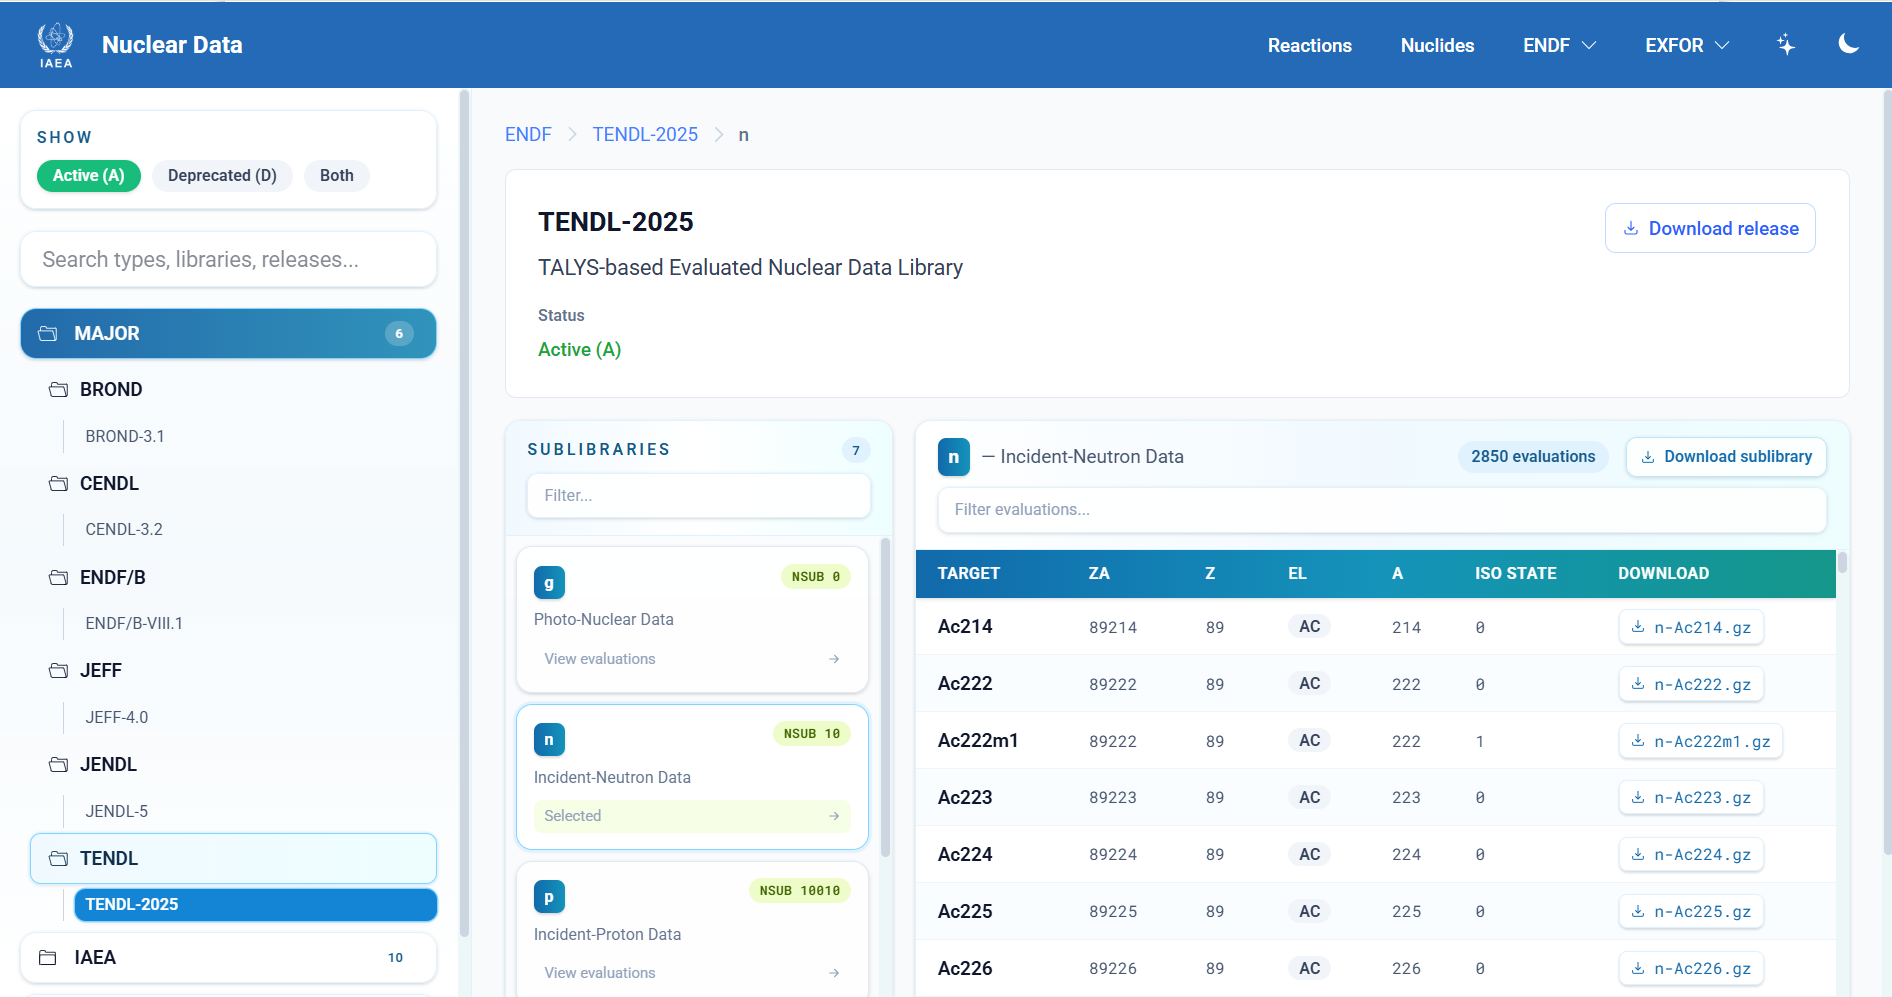
\includegraphics[width=0.75\linewidth]{figures/Screenshot 2026-10-29 145841.png}
    \caption{Screenshot of the New ENDF Archive User Interface}
    \label{fig:endf-archive-ui}
\end{figure}

Another feature that was presented was the inclusion of an AI chat agent aimed to take user questions related to nuclear reactions in natural language and make use of the available APIs and data to answer by giving a result list and plotting the data within the same web user interface or by enabling download of the data and plot images in the chat window.

\begin{figure}[H]
    \centering
    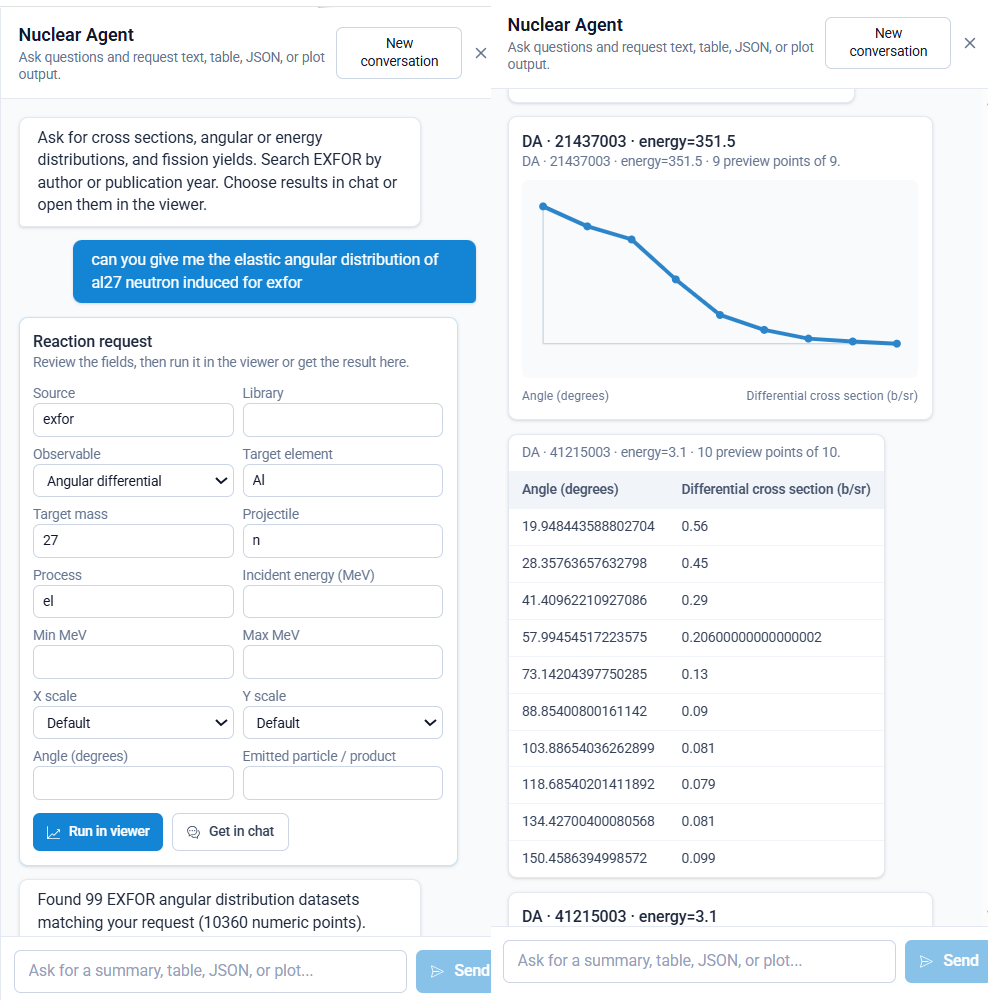
\includegraphics[width=0.75\linewidth]{figures/ai assisstant.png}
    \caption{Screenshot of AI Chat Agent for Experimental and Evaluated Nuclear Data}
    \label{fig:ai-chat-agent}
\end{figure}




\subsection{Wednesday, 28 October 2026}

\subsubsection{ENDF modernization efforts: endf-parserpy and endf-userpy\\ Georg Schnabel (IAEA)}
% Official contribution: https://conferences.iaea.org/event/498/contributions/43619/
% Scheduled date: 2026-10-28.
\paragraph{Abstract}
% No substantive abstract published at the time of preparation.
\mbox{}

Georg Schnabel briefly presented the IAEA Fusion Evaluated Nuclear Data Library (FENDL)~\cite{Schnabel2024FENDL} as an example to discuss challenges associated with the maintenance and development of large nuclear data library projects with a long history and many contributors. Two key aspects are traceability of changes over time and the reproducibility of derived files, such as specific files for transport codes, e.g. MCNP. Key information technologies adopted by the FENDL project were briefly discussed: Git and GitHub for traceability, git-annex for dealing with many large files, Apptainer for perfect reproducibility of NJOY2016~\cite{NJOY} processing, and the JADE tool for library verification and validation, developed by Fusion For Energy (F4E), United Kingdom Energy Authority (UKAEA) and partners.

Traceability is also improved by translating legacy nuclear data formats to commonly used Internet container and exchange formats, such as the Extensible Markup Language (XML) and JavaScript Object Notation (JSON). Modern tools and programming languages seamlessly support parsing and serializing these formats, which simplifies workflows, the development of new tools and the integration into agentic workflows. At the community level, the adoption of modern formats lowers technological entrance barriers to newcomers and consequently promotes robust and sustainable inter-generational knowledge transfer.

With regard to nuclear reaction data, the General Nuclear Database Structure (GNDS) format~\cite{GNDS2023} is an important modernization project that currently uses XML as a container format. While GNDS will gradually replace the Evaluated Nuclear Data File (ENDF-6) format~\cite{ENDF6FormatsManual2023} for the exchange and dissemination of evaluated nuclear reaction data, ENDF-6 is still widely used by contemporary library projects as well as their previous versions over the last several decades. Seamless access to these data is therefore also paramount to ensure that knowledge from the past remains accessible and can inform future developments. Removing the technological barrier imposed by the ENDF-6 format was the primary motivation for the development of the Python packages endf-parserpy~\cite{endf-parserpy} and endf-userpy~\cite{endf-userpy} at the IAEA Nuclear Data Section so that traceable and reproducible workflows can also integrate evaluated data provided in the ENDF-6 format.

The endf-parserpy package enables low-level parsing of ENDF data and their conversion to nested Python dictionaries, which are first-class citizens in Python and hence powerful functionality to traverse, analyze and modify them is available out-of-the-box. For example, a nested dictionary with ENDF data can be converted to a JSON file in only a couple lines of code, which enables seamless access to ENDF data from many other programming languages and web applications. Furthermore, Python is one of the most prominent languages for Machine Learning (ML) and data science work, which simplifies the integration of ENDF data into data pipelines and ML applications.
As library maintenance also entails fixing and updating evaluated nuclear data occasionally, endf-parserpy also allows for the serialization of Python dictionaries with ENDF data of appropriate structure to ENDF files. By extension, JSON files with ENDF data can be seamlessly serialized to the ENDF format as well. The Python package is available under the permissive MIT license on GitHub at \url{https://github.com/iaea-nds/endf-parserpy} and comprehensive documentation with many tutorials is provided at \url{https://endf-parserpy.readthedocs.io/en/latest/}.

The other Python package, endf-userpy, provides a simple user-interface with a very limited set of high-level functions that return evaluated nuclear data in a form that can be directly compared with experimental data (or is very close to this goal). Examples of quantities of interest are cross sections, angular distributions and double-differential cross sections for both inclusive reactions, e.g. (n,tot) and exclusive ones, e.g. (n,2n). Under the hood, it traverses nested Python dictionaries as produced by endf-parserpy and assembles and interpolates data stored therein as needed to correctly reconstruct the physical quantity queried by the user. An early version for testing (in alpha status) is available at \url{https://github.com/iaea-nds/endf-userpy}. 


\paragraph{Discussion}
% Source: Webex-

ENDF handling through a formal description of the format, low-level parsing and higher-level access to physical quantities. The recipe-based approach supports nested Python structures and generated C++ parsers; endf-userpy builds on these representations to expose observables. Discussion addressed constructing files from tabulated data, combining information from different sections and remaining gaps in convenience functions and covariance handling. Participants distinguished format checks from physical validation. Issue reports, examples and contributions were discussed as ways to improve the tools and support their maintenance. 


\subsubsection{Modernizing ENSDF with REST APIs and Physics-Informed AI\\ Donnie Mason (BNL)}
% Official contribution: https://conferences.iaea.org/event/498/contributions/43627/
% Scheduled date: 2026-10-28.
\paragraph{Abstract}
The Evaluated Nuclear Structure Data File (ENSDF)~\cite{ENSDF_Manual} is a foundational resource for nuclear structure
and decay information, providing evaluated data that support research across nuclear physics, nuclear energy, astrophysics, medicine, and national security. As experimental measurements continue
to grow in volume and complexity, new approaches are needed to improve both access to ENSDF and the efficiency of the evaluation process. The National Nuclear Data Center (NNDC) at Brookhaven National Laboratory is pursuing these goals through the modernization of ENSDF data services and the use of physics-informed artificial intelligence in nuclear data evaluation. 
\begin{figure}[htbp]
    \centering  
    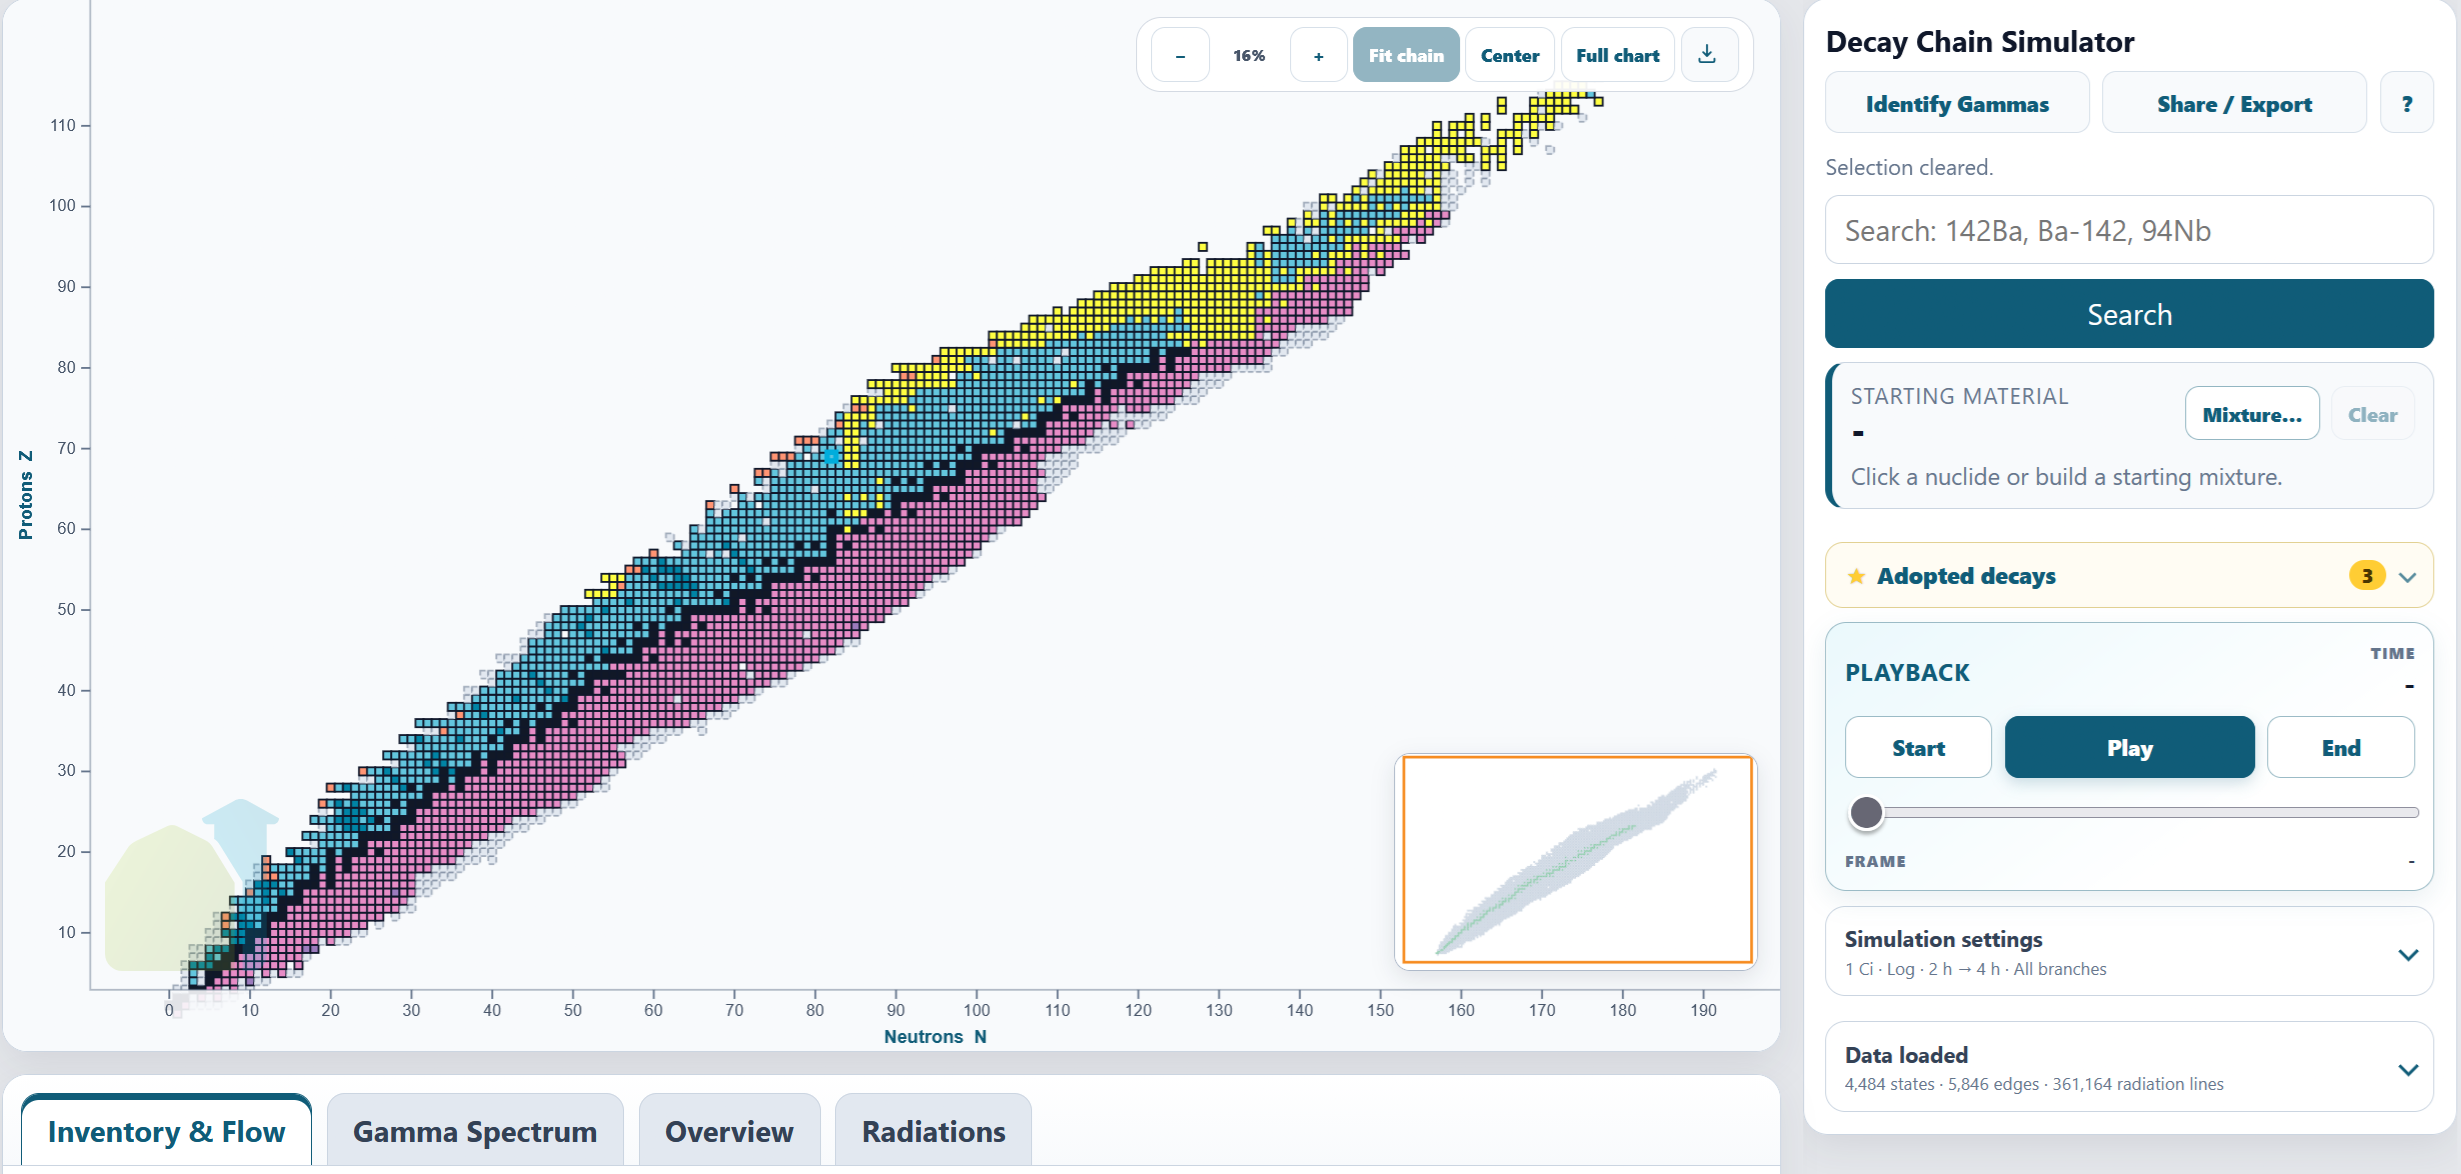
\includegraphics[width=.9\textwidth]{figures/mason_ss_1.png}
    \caption{Decay chain simulator featuring interactive chart of nuclides}
    \label{fig:submission_form}
\end{figure}
This talk will introduce the new ENSDF REST API~\cite{ensdf_api}, which provides standardized, programmatic access to evaluated nuclear structure and decay data and is publicly available at \url{https://www.nndc.bnl.gov/ensdf-api/}. The API makes ENSDF available to modern
scientific workflows, analysis software, web applications, and computational tools, and provides a foundation for new applications built around evaluated nuclear data.
With the addition of modernized access to nuclear data, interactive web applications are being developed. 
\begin{figure}[htbp]
    \centering  
    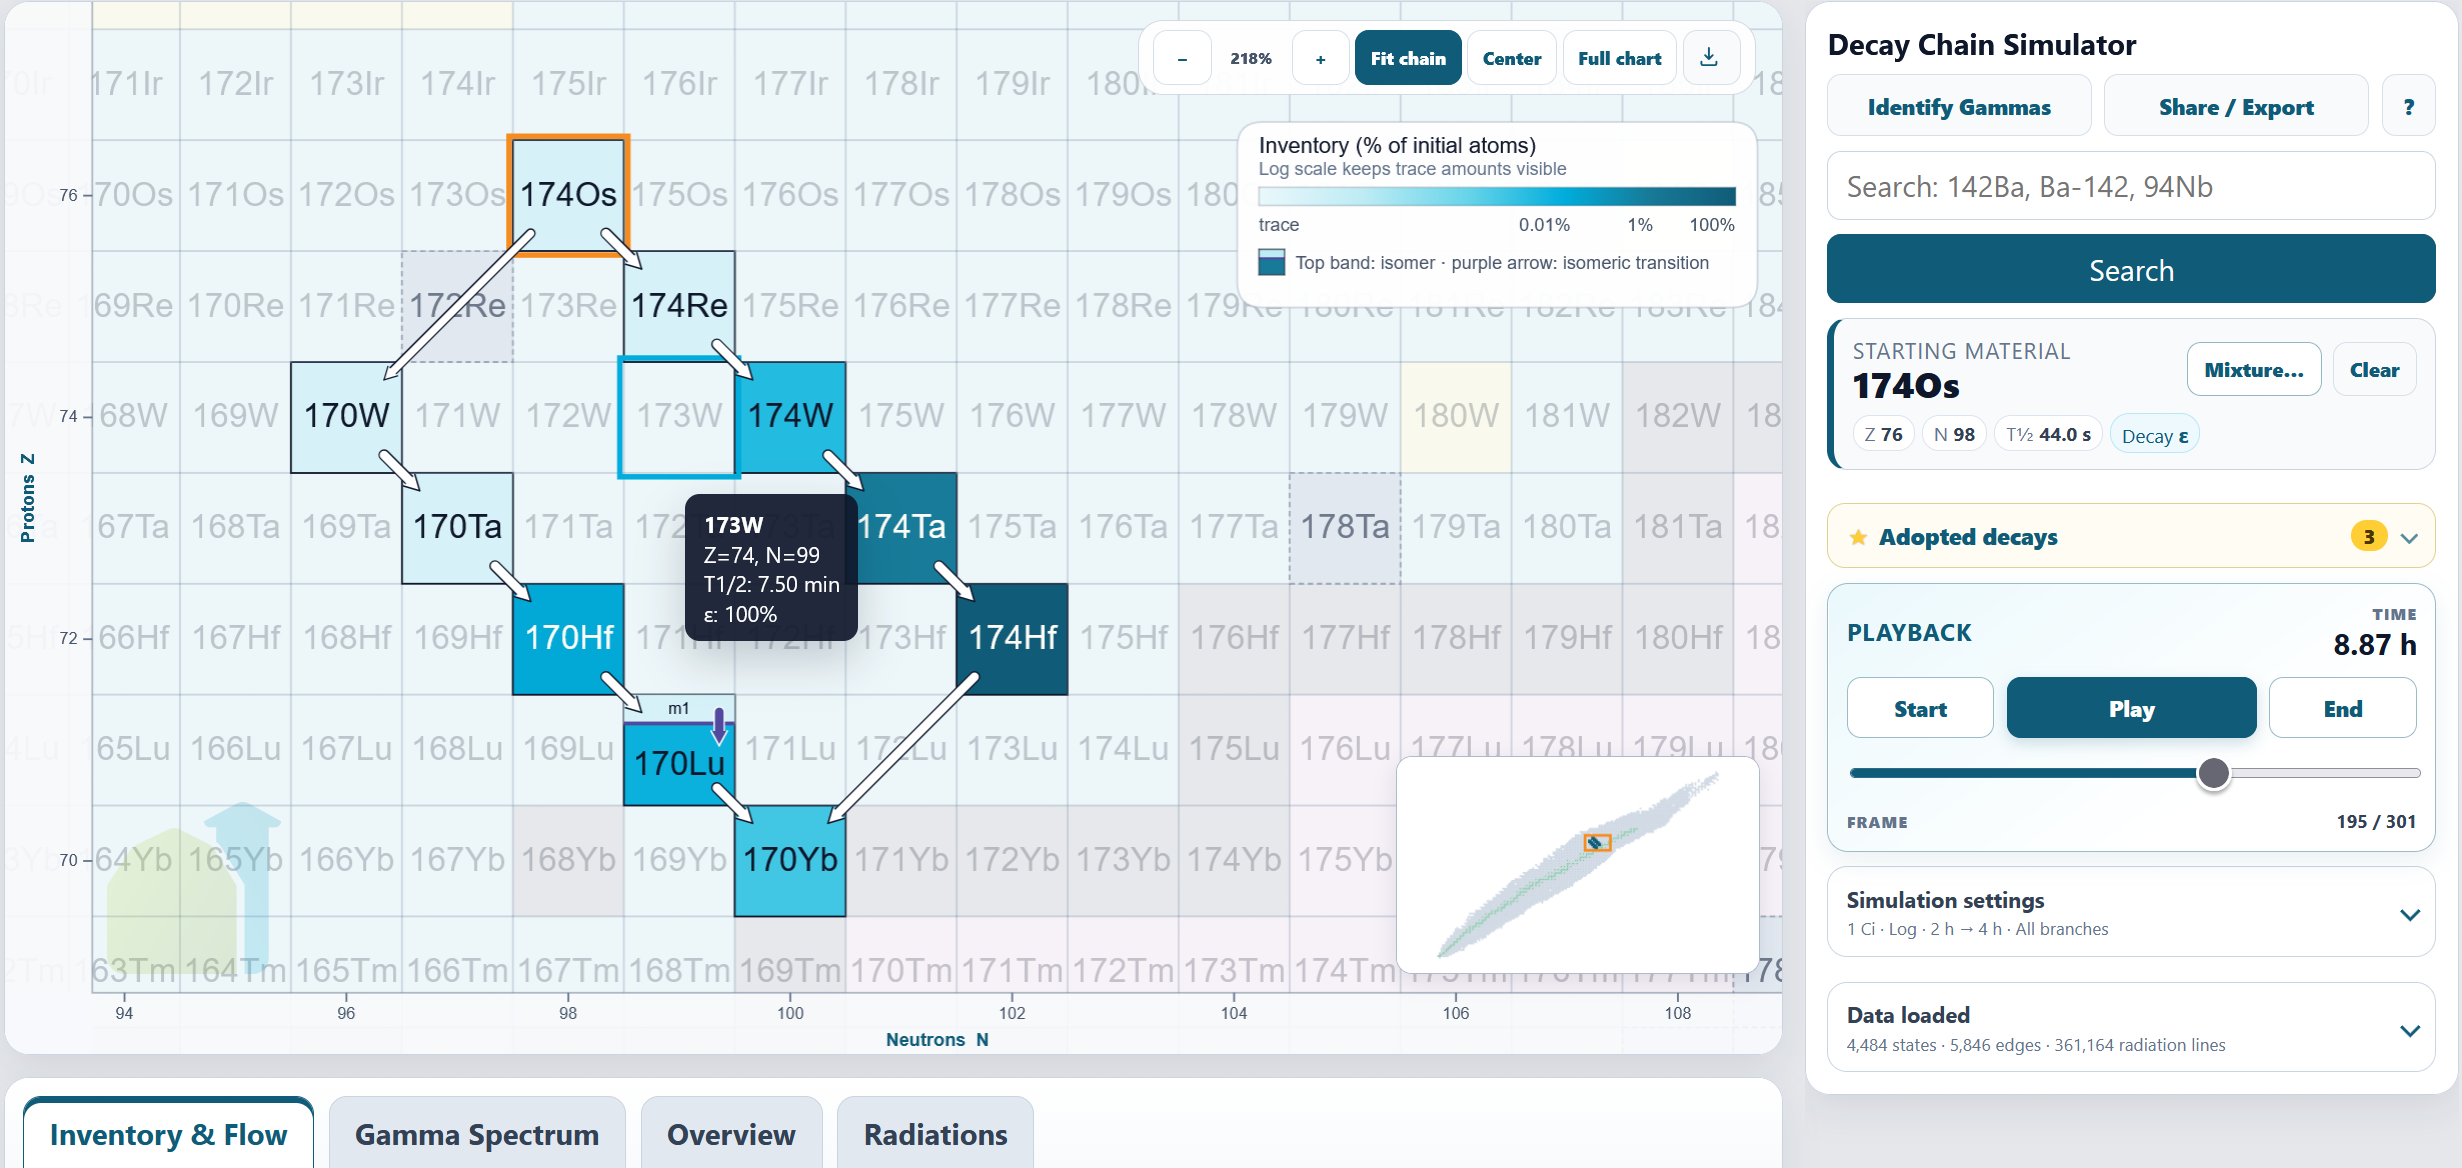
\includegraphics[width=.9\textwidth]{figures/mason_ss_2.png}
    \caption{Selecting a nuclide displays the entire chain and time controls are used to visualize the inventory over time.}
    \label{fig:submission_form}
\end{figure}
As part of the Adopted Decay project, we have implemented an interactive decay chain simulator.
The talk will also describe a newly funded effort supported through the U.S. Department of Energy’s Genesis Mission, a national initiative focused on using artificial intelligence to accelerate scientific
discovery. As part of this effort, the NNDC is investigating the use of physics-informed AI to assist with ENSDF evaluations while retaining expert oversight and the provenance and traceability required for evaluated nuclear data.
Four initial tasks have been identified: measurement reconciliation, using inference to compare
experimental measurements and determine consistent adopted values; J$\pi$  assignment, using classification to assist with nuclear spin and parity assignments; multipolarity assignment, using experimental observables and nuclear-structure information to identify transition multipolarities; and
anomaly detection, identifying unusual or potentially inconsistent data for further investigation by
evaluators.
Together, the ENSDF REST API and the Genesis Mission AI effort provide complementary approaches to modernizing ENSDF. The API provides programmatic access to the evaluated data, while the AI effort explores ways to make the evaluation process more efficient and help evaluators
handle increasingly large and complex datasets.
\begin{figure}[htbp]
    \centering  
    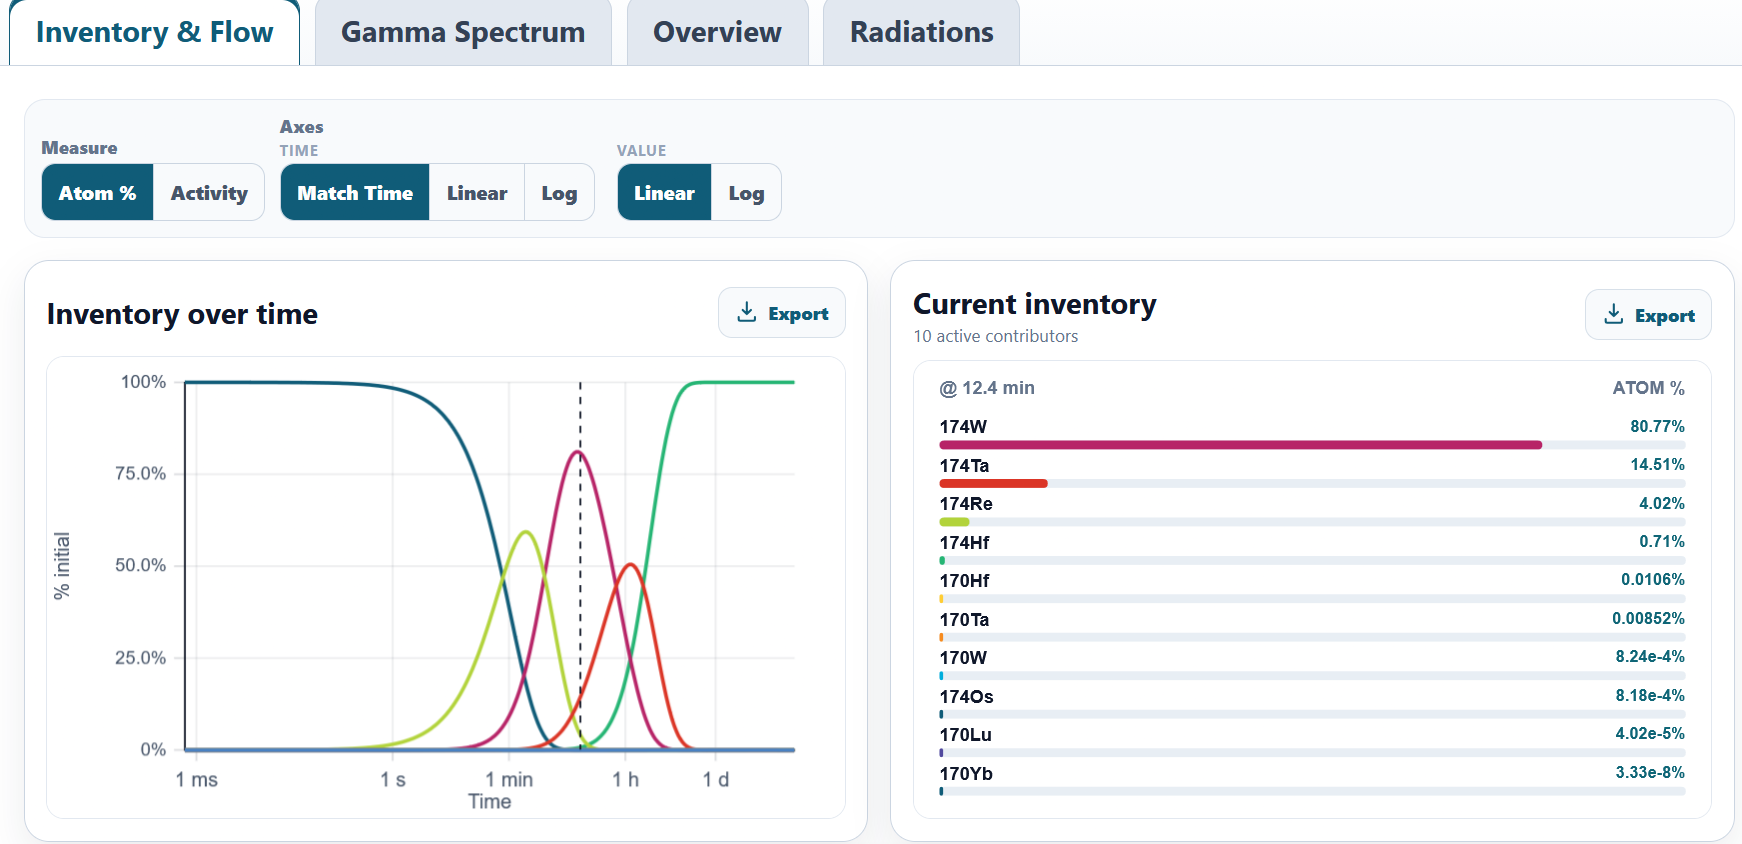
\includegraphics[width=.9\textwidth]{figures/mason_ss_3.png}
    \caption{Addition plots tracking inventory over time, current inventory, and even gamma spectra is provided.}
    \label{fig:submission_form}
\end{figure}


\paragraph{Discussion}
Donnie Mason presented REST APIs for NNDC databases. The APIs for ENSDF, ENDF and CapGam APIs are available now, and NuDat and Wallet Cards APIs are coming soon. He overviewed the Adopted Decay web application to simulated ENSDF decay data directly in a browser. Discussion covered selective retrieval, evaluation cutoff dates, and the provenance of adopted datasets. Mason then described the Genesis Mission project (St. Joseph’s University and BNL), which is developing physics-informed AI for four parts of evaluation: recommended values, multipolarities, spin-parity and anomaly detection. The approach is that AI proposes, deterministic tools decide, and evaluators make the final call. Schema references, explicit uncertainty representations, and reusable computational functions were discussed as further improvements.




\subsubsection{Starrydata\\ Yukari Katsura (NIMS)}
% Official contribution: https://conferences.iaea.org/event/498/contributions/43632/
% Scheduled date: 2026-10-28.
\paragraph{Abstract}
% No substantive abstract published at the time of preparation.
This talk introduces the development of Starrydata\cite{Katsura2025Starrydata}, a web-based materials property database, and shares insights from the data collection project that may be useful for similar initiatives in other research fields. Starrydata facilitates the manual extraction of numerical data from figures in scientific publications, particularly temperature-dependent thermoelectric properties. The database currently contains over 230,000 curves from more than 100,000 samples, extracted from over 66,000 figures in 17,000 scientific papers.

The largest datasets cover thermoelectric, magnetic, battery, and dielectric materials. The data collection process begins with designing a data schema and selecting target figures. Based on a list of DOIs obtained from external databases, data collection pages are automatically generated by retrieving bibliographic information from Crossref. Data collection is performed by dedicated curators, who label graph axes, trace data points, annotate sample information, and merge records corresponding to identical samples appearing in multiple figures within the same paper.

Automated data extraction methods are also under development. LLM-assisted extraction has been implemented to retrieve sample information from the experimental methods sections of scientific papers. LLMs are also used in Starrydata Auto-summary GPT, a custom GPT built on ChatGPT that summarizes the research scope, figures, samples, and experimental methods from uploaded PDF files. However, the use of LLMs is currently restricted to open-access papers published under the CC BY license. Consequently, manual data curation by dedicated curators remains the primary approach for covering a broad range of published literature.

Using the collected data, visualization tools have been developed, including composition maps, property curves, and scatter plots, to explore relationships between material compositions and thermoelectric properties. The Starrydata web system is publicly available at \url{https://starrydata.nims.go.jp}, and the entire dataset is available for download. Data collection activities are financially supported through collaborations with industrial partners interested in utilizing published research data. This talk also discusses strategies for organizing data collection teams and integrating large language models (LLMs) into the data collection workflow.
\mbox{}\par
\begin{figure}
    \centering
    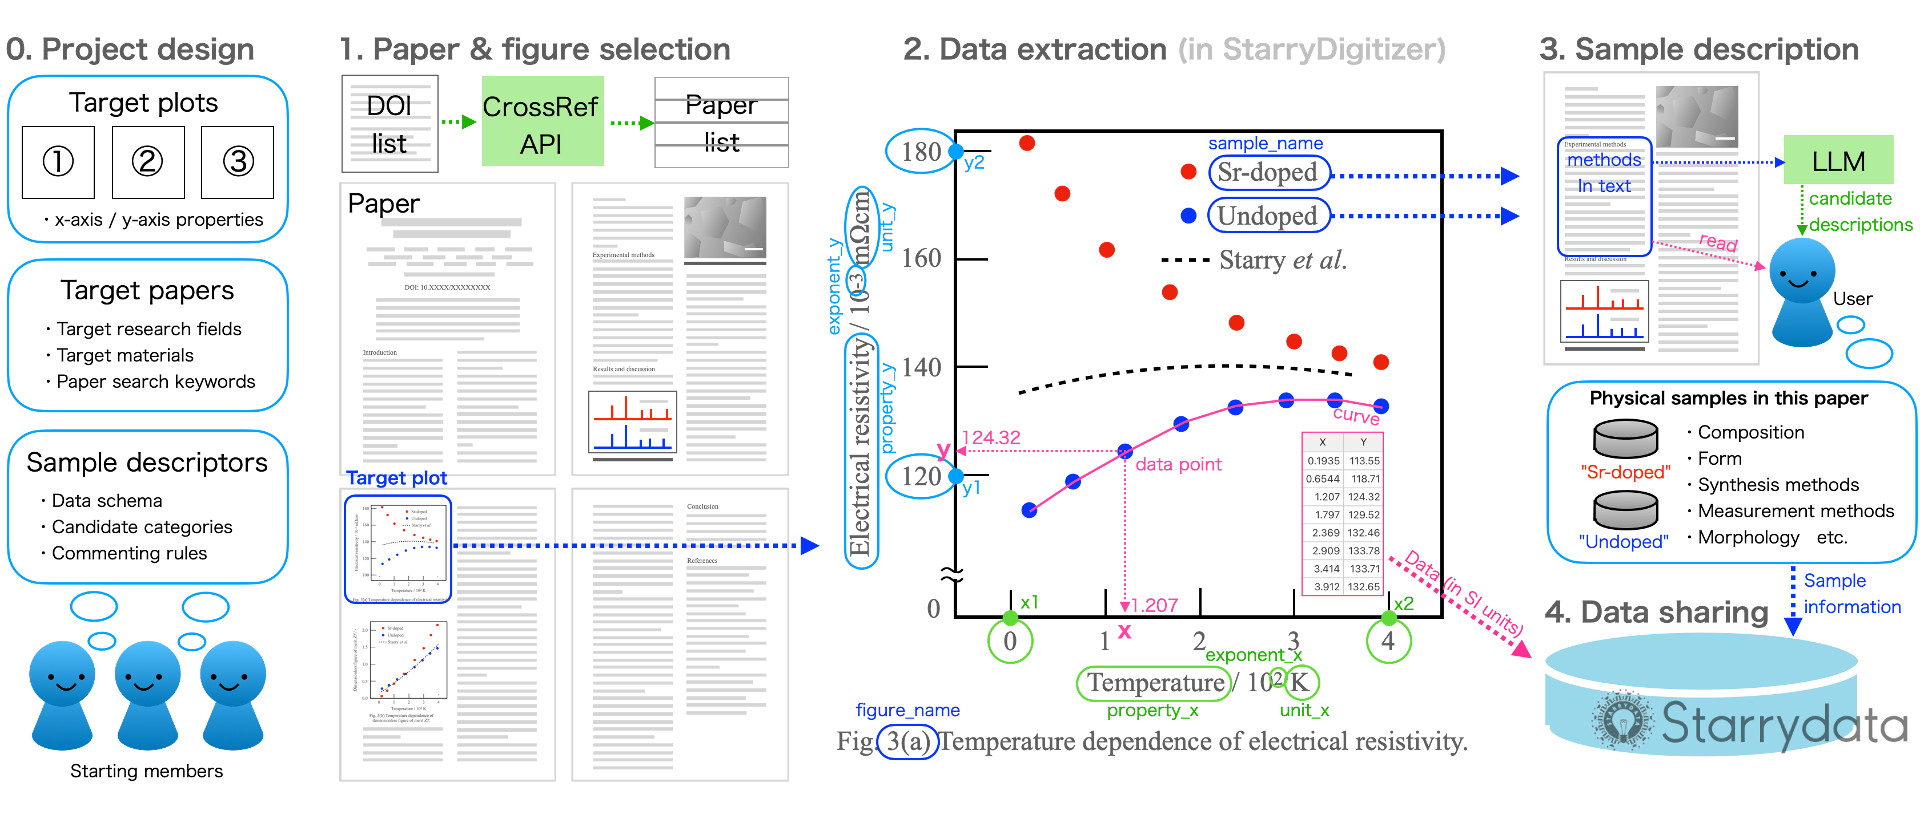
\includegraphics[width=1\linewidth]{figures/Figure1.png}
    \caption{Data collection process in Starrydata.\cite{Katsura2025Starrydata}}
    \label{fig:starrydata-collection}
\end{figure}


\paragraph{Discussion}
% Source: Webex-Summary/day1.pdf; use the meeting date, not the filename.
Yukari Katsura presented Starrydata's collection of numerical materials data from published figures, with sample metadata and links to source articles. The presentation described curation tools, manual digitisation and assisted extraction. Discussion covered overlapping traces, figure quality, digitisation errors and the limits of automation. Language models were considered for metadata preparation with human checking. Participants also discussed sustaining curation, discovering available properties and connecting experimental records to other materials resources. The examples offered experience relevant to literature-based nuclear data collection, while differing sample definitions and data models complicate direct integration.


\subsection{Thursday, 29 October 2026 (scheduled)}

\subsubsection{Towards Agentic Nuclear Data: AI/ML in the Nuclear Decay Data and Fusion Data Pipeline\\ Dragan Avramovski (IAEA)}
% Official contribution: https://conferences.iaea.org/event/498/contributions/43622/
% Scheduled date: 2026-10-29.
\paragraph{Abstract}
% No substantive abstract published at the time of preparation.
This joint presentation introduces two AI agents under development at the IAEA Nuclear Data Section. The first automates the processing and validation of nuclear structure and decay data in the ENSDF\cite{ENSDF_Manual} pipeline behind LiveChart\cite{livechart}, and expands data APIs for external users. The second is a fusion data agent that helps users find and query fusion-related data. Both use AI and ML methods and lay the groundwork for agentic software that can query and synthesize nuclear data on its own.
\mbox{}\par

\paragraph{Discussion}
% Source: Webex-Summary/day3.pdf; meeting date 29 October 2026.
% The supplied summary covers Dragan Avramovski's presentations but
% incorrectly attributes them to Shin Okumura. Action assignments are unverified.
Dragan Avramovski outlined proposed agent-assisted workflows for nuclear structure and decay data and for fusion data, building on existing processing scripts. Discussion focused on combining fixed processing steps with limited agent autonomy, verification and final human review. An orchestrator would coordinate extraction, validation and reporting, with executor and verifier roles and a record of changes. AI agents powered by LLMs can efficiently synthesize data and produce precise, tailored reports from large volumes of log data. Suggested HTML reports would let reviewers inspect differences between releases and trace values to their sources. Machine-learning anomaly scores would flag records for review. Participants also distinguished internal production workflows from public-facing data assistants, which raise additional questions about trust and provenance. These were design proposals, rather than a completed pipeline.


\subsubsection{Agentic AI Engineering with Local Models\\ Dragan Avramovski (IAEA)}
% Official contribution: https://conferences.iaea.org/event/498/contributions/43623/
% Scheduled date: 2026-10-29.
\paragraph{Abstract}
% No substantive abstract published at the time of preparation.
Large language models do much more when they work through a task in steps instead of answering in one go. This lecture introduces agentic AI workflows and it covers the four main design patterns: reflection, tool use, planning and multi-agent collaboration. The examples show why the design of the workflow can matter more than the size of the model. The lecture also focuses on the practical side of building agents. The final part shows some aspects on ways of running local models.
\mbox{}\par

\paragraph{Discussion}
% Source: Webex-Summary/day3.pdf; meeting date 29 October 2026.
% Speaker names in the automatic summary are unreliable; no inferred
% commitments, delivery dates or hardware benchmarks are adopted here.
Dragan Avramovski discussed the design of agents, using deterministic checks, verification of intermediate outputs and reversible changes. Participants considered log summarisation and reports highlighting anomalies useful applications for human review. A versioned collection of human-approved examples was proposed for retrieval-augmented generation, allowing corrections to inform later tasks without retraining the model.

Local deployment was discussed in terms of privacy, cost and reproducibility. Quantisation can reduce model memory requirements, while context length and processing speed constrain what existing hardware can support. Discussion also covered prompt injection and risks associated with tool access and communication between agents. Restricted permissions, isolated execution and escalation to a human reviewer were proposed safeguards. Model choice and resource requirements remained matters for testing against specific tasks.


\newpage
\section{Summary of discussions and recommendations}
% Provisional synthesis of 27--28 October 2026 only.
% Webex-Summary/day2.pdf = 27 October; day1.pdf = 28 October.

The discussions concerned practical connections between data services, reuse of software and the interpretation of the data exposed to users. The following synthesis records topics and suggestions from those sessions. Final conclusions and follow-up actions remain open until the meeting is completed.

\subsection{Shared components and developer collaboration}
% Sources: 27 October, Schema/API, visualization continuity and Interoperability;
% 28 October, Schema sharing and Back-end design. NEA slides corroborate principles.
Participants compared independently developed retrieval systems and identified opportunities to share smaller components rather than entire applications. Examples included reaction-string interpretation, human-readable labels, uncertainty objects and schema modules. Common APIs and exchange structures could connect services with different internal implementations. NEA examples illustrated version-controlled contributions, automated validation and links between data releases and persistent identifiers.

Discussion also concerned continuity of services and the effort required to maintain them. Practical exchanges between developers, clear documentation and user feedback were considered useful for sharing knowledge. The group discussed how contributors unfamiliar with Git could take part without needing to understand the full development infrastructure.

\subsection{Structured metadata and experimental-data submission}
% Source: 27 October, Template submission form pilot, Uncertainty representation,
% Integration/automation/APIs and Metadata completeness.
The EXFOR submission prototype combined a graphical form, JSON Schema validation and a review workflow. Participants discussed balancing ease of submission with the metadata needed to interpret measurements. Requirements included experimental conditions, standards, uncertainty sources and correlations, with modular sections for different measurements and support for existing tabular data.

Form completion and schema validation do not by themselves complete compilation or scientific review. Authentication, storage, review responsibilities and integration into the compilation workflow remained questions for further development. DOI-based metadata lookup, clearer onboarding instructions and additional community testing were discussed as ways to reduce contributor effort.

\subsection{Processing, provenance and scientific checks}
% Sources: 27 October, Database exports/provenance and Processing;
% 28 October, CM-to-lab, Conversion transparency and Master-file discrepancies.
Discussion emphasized that comparisons between experimental results and evaluated libraries are reproducible only if the transformations applied to the data are documented along with the source data. Reconstruction, interpolation, units, frame conversions and bin definitions can all change a result. Participants asked for clearer descriptions of the processing behind plotted quantities and exports, including source versions and conversion-code versions, so that any displayed or downloaded result can be regenerated exactly. Downloaded data should also make it possible to understand why apparently equivalent results differ between services.


Participants noted that when several versions of a source dataset are in use, it can be unclear which version a given result comes from. Differences in deleted, empty, duplicate or superseded records then lead to different results.
A traceable provenance of data source is very important to give certainty and confidence in what the data mean and how they can be used. Because several sources of related data may exist, it is paramount that detailed provenance information is accurate and easily accessible by everyone. Provenance information should be provided in standardized and broadly adopted formats.

\begin{itemize}
  \item \textbf{Traceable provenance:} link every result to its specific source version and processing-code version.
  \item \textbf{Version identification:} label each dataset release clearly so users can confirm which one they are using.
  \item \textbf{Programmatic comparison:} compare sources automatically so discrepancies are flagged for review.
  \item \textbf{Layered validation:} combine unit tests and schema validation with physical checks and comparison against reference data.
  \item \textbf{Confidence indicators:} define and test automated indicators for displayed results.
\end{itemize}

% Differences between EXFOR source files and record counts raised questions about deleted, empty, duplicate and superseded records. These affect whether results can be reproduced across services and over time. Programmatic comparison of sources was suggested to reveal discrepancies for review. No common reconciliation rule was established. Unit tests and schema validation were distinguished from physical checks and comparison with reference data: the first two confirm that software behaves consistently, while only the latter two confirm that the results are physically correct. Automated confidence indicators for displayed results remained a proposal requiring definition and testing.


\subsection{APIs, interfaces and access}
% Sources: 27 October, Data Explorer and NEA retrieval demonstrations;
% 28 October, API access/rate limits, Observables UI and Visualization scope.
Demonstrations illustrated programmatic retrieval alongside interactive plots. Discussion addressed discovering available observables, choosing sensible defaults, retaining user controls and linking views back to original records. Selective queries and exports were useful for downstream analysis; bulk downloads raised storage and hosting questions.

Participants discussed the effect of bot protection and rate limits on legitimate API use. API keys, caching and clearer access guidance were considered possible approaches. User-upload comparisons also prompted discussion of client-side processing and temporary storage. These options remained subject to implementation and institutional arrangements; an unrestricted submission or upload service was not established during the recorded sessions.

\subsection{Schemas, curation and AI-assisted workflows}
% Sources: 27 October, Autoscripts, Quality scoring and AI-assisted determinism;
% 28 October, ENSDF/Genesis, Starrydata and Schema header/provenance linking.
ENSDF discussions highlighted explicit representations of values, uncertainties, limits and ranges. Participants proposed including links to the applicable schema and its version in distributed records. Shared schema components and reusable computational functions could support multiple interfaces, while maintaining a distinction between data conversion and interpretation.

The Autotalys and ENSDF presentations explored automation and AI assistance in different parts of the workflow. Discussion favored checking generated routines and retaining explanations and provenance for derived results. Statistical outliers need interpretation; they are not automatically erroneous measurements. Starrydata provided a complementary example of literature-data curation, where extraction tools and language-model assistance still require human checking. Numerical accuracy, source references and the effort needed to sustain curation were recurring concerns.

\subsection{Continuities of modernization efforts}

The continuity and continuous modernization of nuclear data functionalities included in legacy applications and HTML pages, and EXFOR/ENDF interfaces, is important. If a service is discontinued, releasing its source code under an open-source license, enables the community to preserve its functionality, maintain a local version, or develop a successor.



\subsection{Persistent Identification and Versioning of Experimental Data}

Two aspects of persistent identification are important for databases of scientific dataset.

\noindent (1) \textit{Persistent identification of the data themselves.}
Persistent identifiers (PIDs) are essential for the precise citation, traceability, and reproducible reuse of scientific data. Especially for the experimental data, identifying the original publication and identifying the data themselves serve distinct purposes: a publication DOI alone does not necessarily identify the specific dataset or version used in an analysis. Experimental databases therefore need identifiers that allow users to cite the data actually used.

\noindent (2) \textit{Technically sound and coordinated implementation.}
Assigning identifiers alone is insufficient. Effective implementation requires an appropriate granularity of identification, explicit versioning, informative metadata, and persistent resolution to the identified data. Users should be able to identify and access the version they cited, even after the database has been updated. A coherent policy across the institutions maintaining a database is therefore necessary to ensure consistent identification and versioning.

EXFOR provides an important example of both points. Regarding (1), EXFOR does not yet provide complete DOI coverage for the original publications associated with its entries, as also noted in Section~\ref{Pres:SO2}. More fundamentally, precise citation of EXFOR data would require identifiers for individual datasets and their versions, whereas, at present, only the annual EXFOR Master file is assigned a DOI.

Regarding (2), DOIs at the SUBENT level, with distinct identifiers for successive versions, would enable precise identification in a manner comparable to HEPData~\cite{HEPData}, for example \texttt{10.17182/hepdata.183386.v1/t3}. This approach has not yet gained sufficient recognition within the EXFOR community and its responsible agencies. The Data Bank is independently considering the use of Invenio to assign DOIs to new EXFOR entries from its area (area codes \texttt{2} and \texttt{O}). Such initiatives should be guided by a shared identification and versioning policy to ensure consistent and interoperable data citation across EXFOR.

\subsection{Next meeting}
The participants proposed regular follow-up meetings, with annual or biannual exchanges mentioned. The IAEA Nuclear Data Section currently plans to organize the Technical Meeting on Open Experimental and Theoretical Databases and Future Nuclear Data Dissemination Services in 22-26 November 2027.



\newpage

\section*{Declaration of generative AI use}
\addcontentsline{toc}{section}{Declaration of generative AI use}

% AI assistance disclosure. The supplied Webex exports do not identify a
% service version. The author confirmed the drafting model as GPT-6.1 Sol.
% Tool names: https://help.webex.com/article/ne2xaqq/Cisco-AI-Assistant-for-Webex-Suite
% https://developers.openai.com/api/docs/guides/code-generation


% The authors used <ADD AI SERVICE HERE> (Version number XXXXXXXXXXXX) to generate a preliminary transcript of the meeting recording and to help draft the meeting summary that follows. All AI-suggested materials were independently checked, edited, and validated by the authors. No unpublished data, sensitive information, or copyrighted materials were entered into the AI tool. Any use of Artificial Intelligence tools by the authors to support its work is done in a responsible and ethical manner. While AI may have assisted in analysing, drafting, editing or processing content, all outputs were subject to human oversight and review.


\textit{The authors used Cisco AI Assistant for Webex (service version not recorded) to generate preliminary meeting summaries, and OpenAI Codex (GPT-6.1 Sol) to assist with drafting and editing this report. All AI-assisted text is subject to review, correction and approval by the authors, who retain responsibility for the final report. }


\newpage

\phantomsection
\addcontentsline{toc}{section}{References}
\bibliographystyle{unsrt2authabbrvpp}
\bibliography{reference}
\newpage

%%% Appendices

\begin{appendices}
 \section{List of participants}\label{app:participants}
 \begin{center}
{\normalfont\bfseries\fontsize{14pt}{16pt}\selectfont
\meetingsubject\\}
\meetingdate
\end{center}

\begin{longtable}{@{}p{4.5cm}p{\dimexpr\textwidth-4.5cm-2\tabcolsep\relax}@{}}
\toprule
\textbf{Name} & \textbf{Affiliation} \\
\midrule
\endfirsthead
\toprule
\textbf{Name} & \textbf{Affiliation} \\
\midrule
\endhead
\bottomrule
\endlastfoot

% Benjamin Shu & Brookhaven National Laboratory \\
% David Brown & Brookhaven National Laboratory \\
Yukari Katsura & National Institute for Materials Science, Japan \\
Donnie Mason & Brookhaven National Laboratory, USA \\
Anastasia Georgiadou & OECD / NEA Data Bank \\
Julia Sprenger & OECD / NEA Data Bank \\
Dragan Avramovski & IAEA\\
Arjan Koning & IAEA\\
Alejandra Martinez & IAEA\\
Shin Okumura & IAEA\\
Georg Schnabel & IAEA\\
\end{longtable}


  \newpage
 \section{Agenda}\label{app:agenda}
 \begin{center}
{\normalfont\bfseries\fontsize{14pt}{16pt}\selectfont Agenda\\}
\meetingdate
\end{center}
All times are local to Vienna (CET, UTC+1). 

\begingroup
\small
\begin{longtable}{@{}p{2.3cm}>{\raggedright\arraybackslash}p{\dimexpr\textwidth-5.7cm-4\tabcolsep\relax}>{\raggedright\arraybackslash}p{3.4cm}@{}}
\toprule
\textbf{Time} & \textbf{Presentation or activity} & \textbf{Speaker(s) / author(s)} \\
\midrule
\endfirsthead
\toprule
\textbf{Time} & \textbf{Presentation or activity} & \textbf{Speaker(s) / author(s)} \\
\midrule
\endhead
\midrule
\multicolumn{3}{r}{\textit{Continued on the next page}} \\
\endfoot
\bottomrule
\endlastfoot
\multicolumn{3}{@{}l}{\bfseries Tuesday, 27 October 2026} \\*
\midrule
10:00--10:30 & Opening remarks and administrative matters & Arjan Koning \\
10:30--11:00 & Nuclear Data Retrieval, Dissemination, and Data Portals & Shin Okumura \\
11:00--12:00 & Updates on IAEA Nuclear Reaction DataExplorer Developments & Shin Okumura \\
12:00--13:30 & Lunch break &  \\
13:30--14:30 & Strengthening Collaboration and Reproducibility in the Nuclear Data Community: Challenges and NEA Initiatives & Julia Sprenger \\
14:30--15:30 & EXFOR Streamlined Reaction Data Submission & Anastasia Georgiadou and Julia Sprenger \\
15:30--16:00 & Coffee break &  \\
16:00--17:00 & Autotalys nuclear data pipeline with GitHub, ChatGPT and Codex & Arjan Koning \\
17:00--18:00 & Progress in the Development of the New Nuclear Data Retrieval System & Alejandra Martinez \\
\midrule
\multicolumn{3}{@{}l}{\bfseries Wednesday, 28 October 2026} \\*
\midrule
10:00--11:00 & endf-parserpy and endf-userpy & Georg Schnabel \\
11:00--12:00 & Modernizing ENSDF with REST APIs and Physics-Informed AI & Donnie Mason \\
12:00--13:30 & Lunch break &  \\
13:30--14:30 & Starrydata & Yukari Katsura \\
14:30--16:30 & Discussion & All \\
\midrule
\multicolumn{3}{@{}l}{\bfseries Thursday, 29 October 2026 (scheduled)} \\*
\midrule
10:00--11:00 & Towards Agentic Nuclear Data: AI/ML in the Nuclear Decay Data and Fusion Data Pipeline & Dragan Avramovski \\
11:00--12:00 & Agentic AI Engineering with Local Models & Dragan Avramovski \\
12:00--13:30 & Lunch break &  \\
13:30--13:40 & Photo session&  \\
14:00--17:00 & Discussion & All \\
\midrule
\multicolumn{3}{@{}l}{\bfseries Friday, 30 October 2026 (scheduled)} \\*
\midrule
10:00--12:30 & Compilation of meeting report & All \\
\end{longtable}
\endgroup

Source: \url{https://conferences.iaea.org/event/498/timetable/}.


\end{appendices}
\newpage
%%% Back page

\thispagestyle{empty}
%% please add the blank pages to finish the report with even page number 
\mbox{}\newpage
\thispagestyle{empty}
\mbox{}\newpage

\thispagestyle{empty}
~ \vspace{20cm}
\begin{table}[b]
 \begin{center}
 \begin{tabular}{lr}
   \toprule[1pt]
     \begin{minipage}{0.47\linewidth}
     \begin{flushleft}Nuclear Data Section\\International Atomic Energy Agency\\P.O. Box 100\\A-1400 Vienna\\Austria \smallskip \end{flushleft}
   \end{minipage} &
   \begin{minipage}{0.47\linewidth}
     \begin{flushright}e-mail: nds.contact-point@iaea.org\\fax: (43-1) 26007\\telephone: (43-1) 2600 21725 \\Web: http://nds.iaea.org/\end{flushright}
   \end{minipage}\\
  \bottomrule[1pt]
 \end{tabular}
 \end{center}
\end{table}

\end{document}
